\documentclass{beamer}

\usepackage{graphics}
\usepackage{graphicx}
\usepackage{amsmath,amssymb,amsthm}
%\usepackage{subeqnarray}
%\usepackage{easybmat}
%\usepackage{subfigure}



%\usepackage{HA-prosper}
%\usepackage[dvips,letterpaper]{geometry}


\def\R{\mathcal{R}}
\def\D{\mathcal{D}}
\def\C{\mathcal{C}}
\def\IC{\mathbb{C}}
\def\IN{\mathbb{N}}
\def\IR{\mathbb{R}}
\def\IZ{\mathbb{Z}}
\def\Rzero{\mathcal{R}_0}
\def\diag{\textrm{diag}}
\def\tr{\textrm{tr}}
\def\det{\textrm{det}}
\def\sgn{\textrm{sgn}}
\def\imply{$\Rightarrow$}
\def\dbint{\int\!\!\!\int}
\def\dbintb{\mathop{\int\!\!\!\!\int}}
\def\tpint{\int\!\!\!\int\!\!\!\int}

\newtheorem{proposition}{Proposition}

\setbeamertemplate{navigation symbols}{}
\setbeamertemplate{footline}
{%
\quad\insertsection\hfill p. \insertpagenumber\quad\mbox{}\vskip2pt
}

\title[Single population growth]{Single population growth models}
\date{}

\begin{document}

\frame{\titlepage}
%%%%%%%%%%%%%%
%%%%%%%%%%%%%%


\section{Objectives}
\frame{\frametitle{Objective}
We are given a table with the population census at different time intervals between a date $a$ and a date $b$, and want to get an expression for the population. This allows us to: 
\begin{itemize}
\item compute a value for the population at any time between the date $a$ and the date $b$ (\textbf{interpolation}),
\item predict a value for the population at a date before $a$ or after $b$ (\textbf{extrapolation}).
\end{itemize}
}

\frame{
\begin{center}
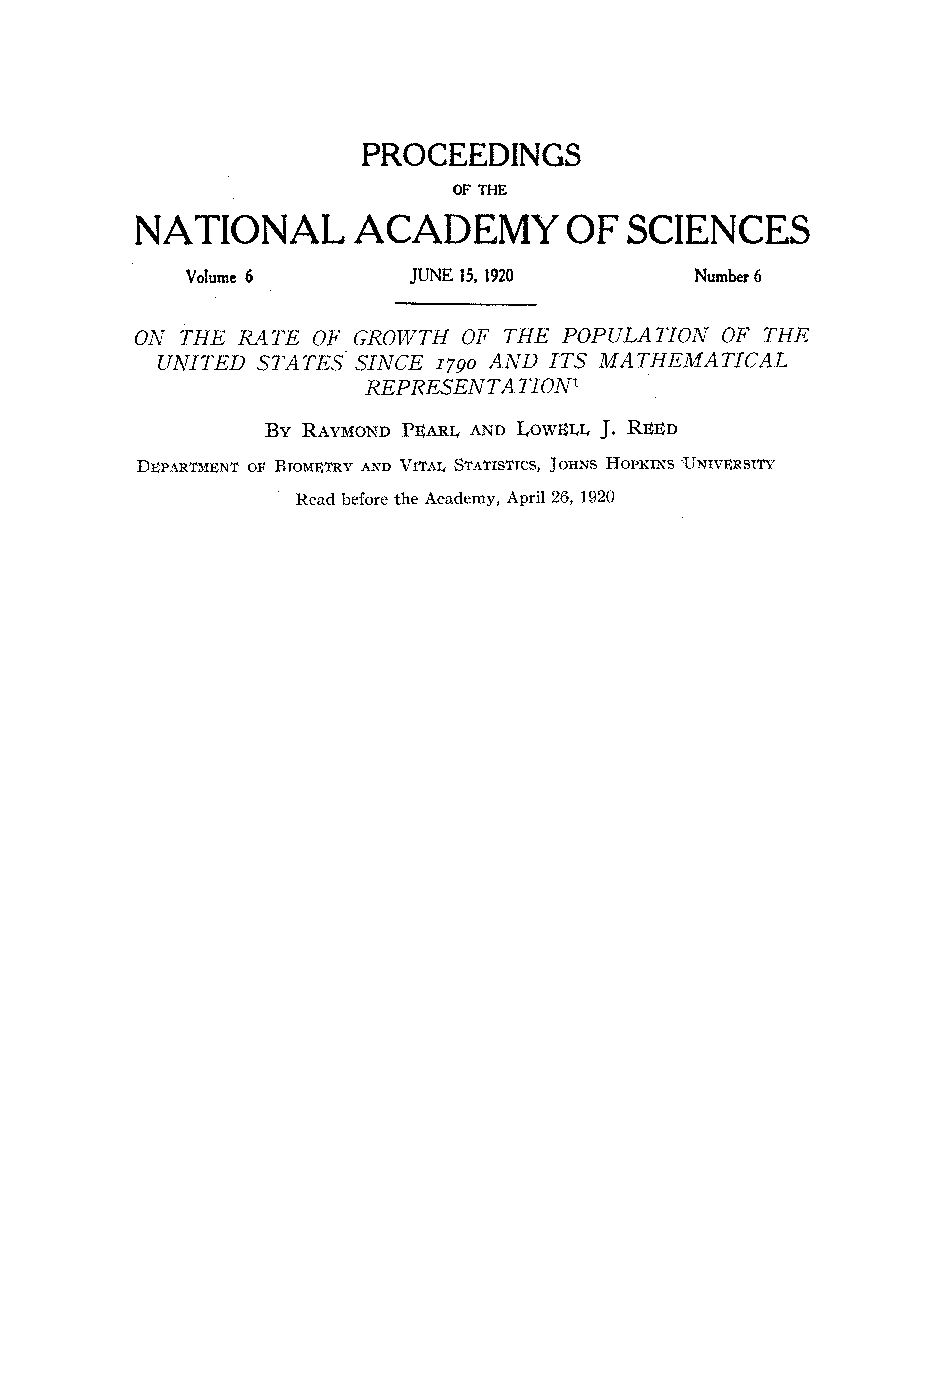
\includegraphics[width=\textwidth]{titre_PearlReed1920PNAS6}
\end{center}
}

\section{The data: US census}

\frame{
\begin{center}
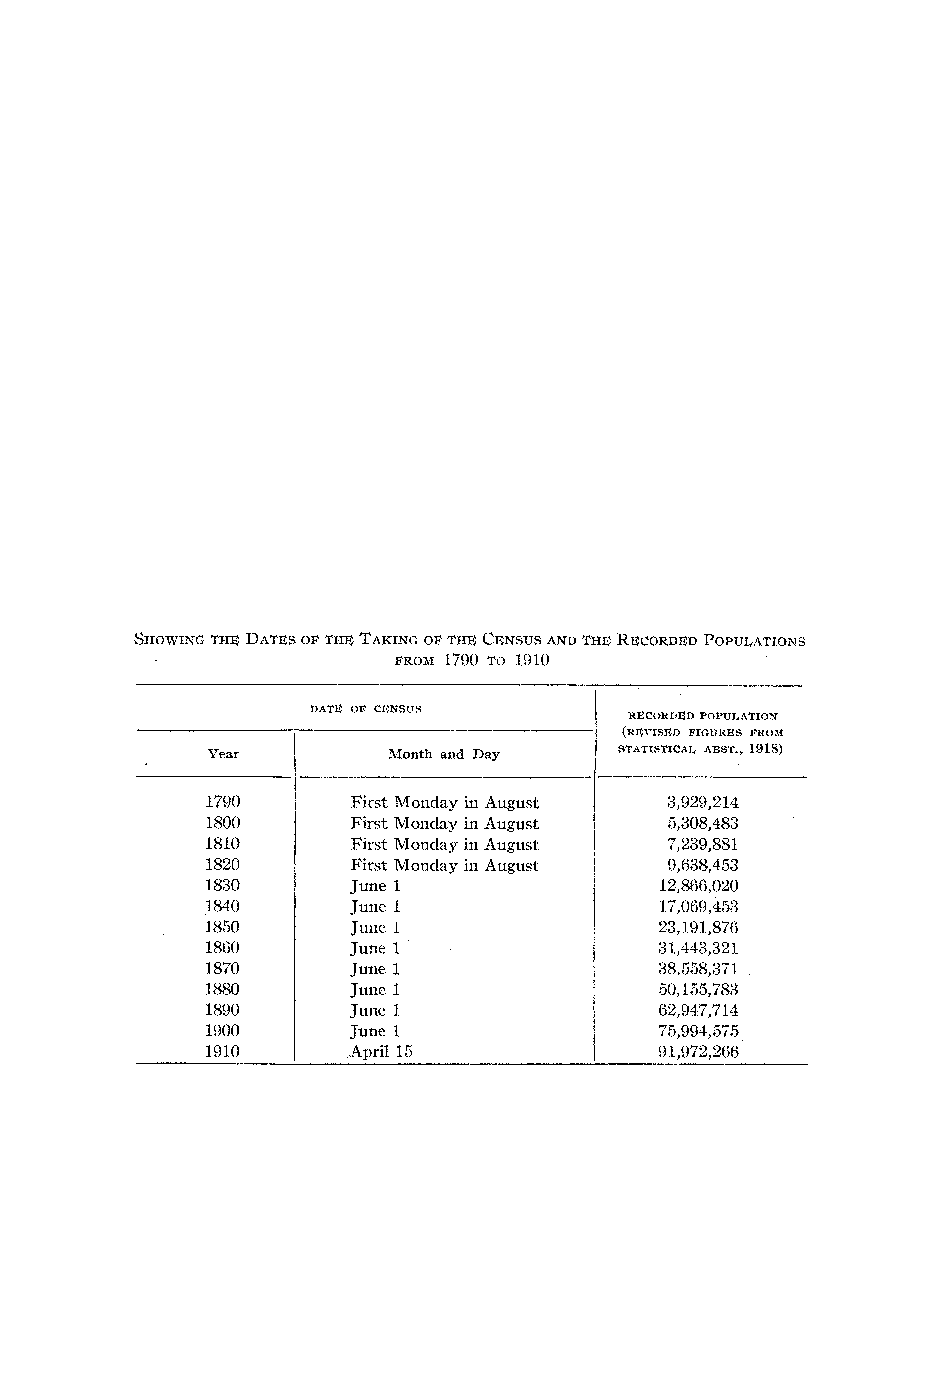
\includegraphics[width=\textwidth]{table_PearlReed1920PNAS6}
\end{center}
}

\frame{\frametitle{The US population from 1790 to 1910}
\begin{center}
\begin{tabular}[t]{cc}
\begin{tabular}{cc}
Year & Population\\
& (millions) \\
\hline
1790 & 3.929 \\
1800 & 5.308 \\
1810 & 7.240 \\
1820 & 9.638 \\
1830 & 12.866 \\
1840 & 17.069 \\
1850 & 23.192
\end{tabular} 
&
\begin{tabular}{cc}
Year & Population \\
& (millions) \\
\hline
1860 & 31.443 \\
1870 & 38.558 \\
1880 & 50.156 \\
1890 & 62.948 \\
1900 & 75.995 \\
1910 & 91.972 
\end{tabular}
\end{tabular}
\end{center}
}


\frame{\frametitle{PLOT THE DATA !!! (here, to 1910)}
Using MatLab (or Octave), create two vectors using commands such as
\vskip0.2cm
{\tt t=1790:10:1910;}\\
Format is
\begin{center}
Vector=Initial value:Step:Final value
\end{center}
(semicolumn hides result of the command.)\\[0.5cm]

{\tt P=[3929214,5308483,7239881,9638453,12866020,...
17069453,23191876,31443321,38558371,50155783,...
62947714,75994575,91972266];}\\[0.5cm]

Here, elements were just listed ({\tt ...} indicates that the line continues below).
}


\frame{
Then plot using \\
{\tt plot(t,P);}
\begin{center}
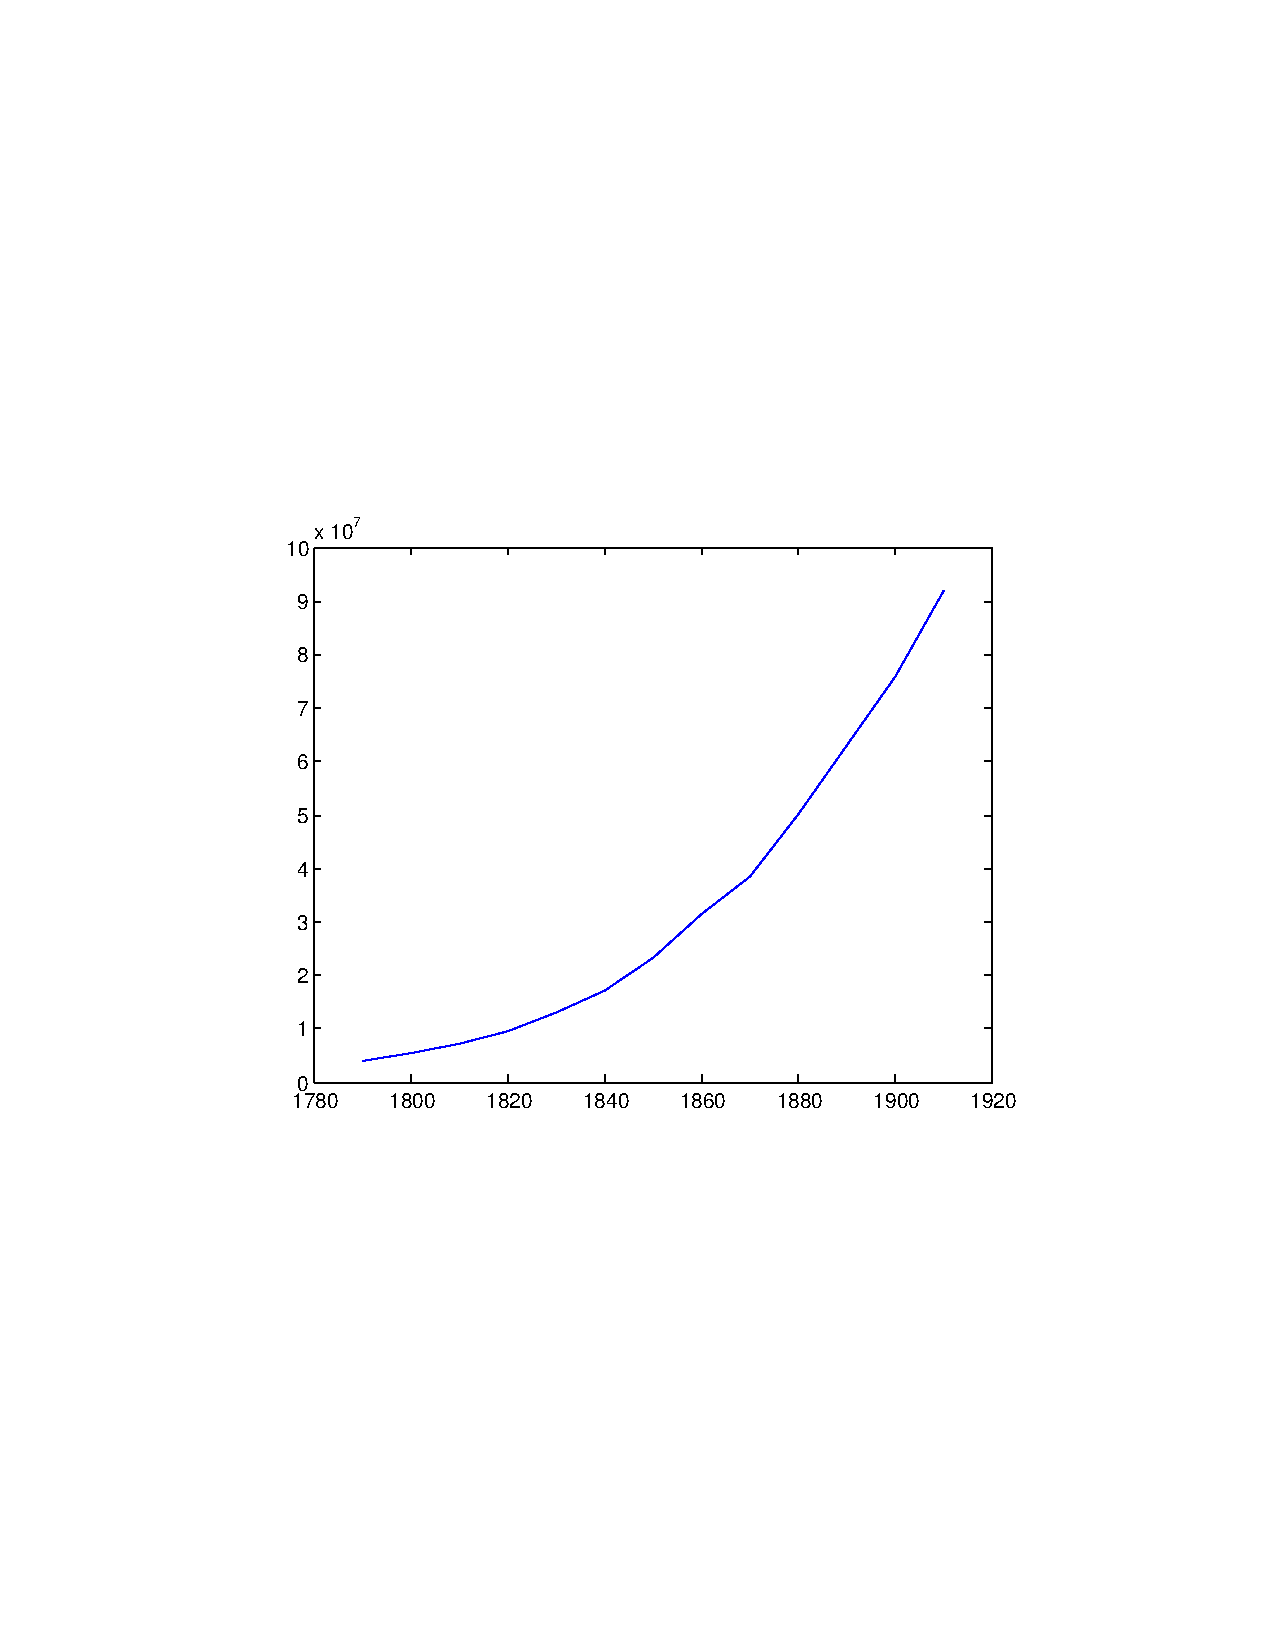
\includegraphics[width=0.9\textwidth]{USpop_to1910}
\end{center}
}

\frame{
To get points instead of a line \\
{\tt plot(t,P,'*');}
\begin{center}
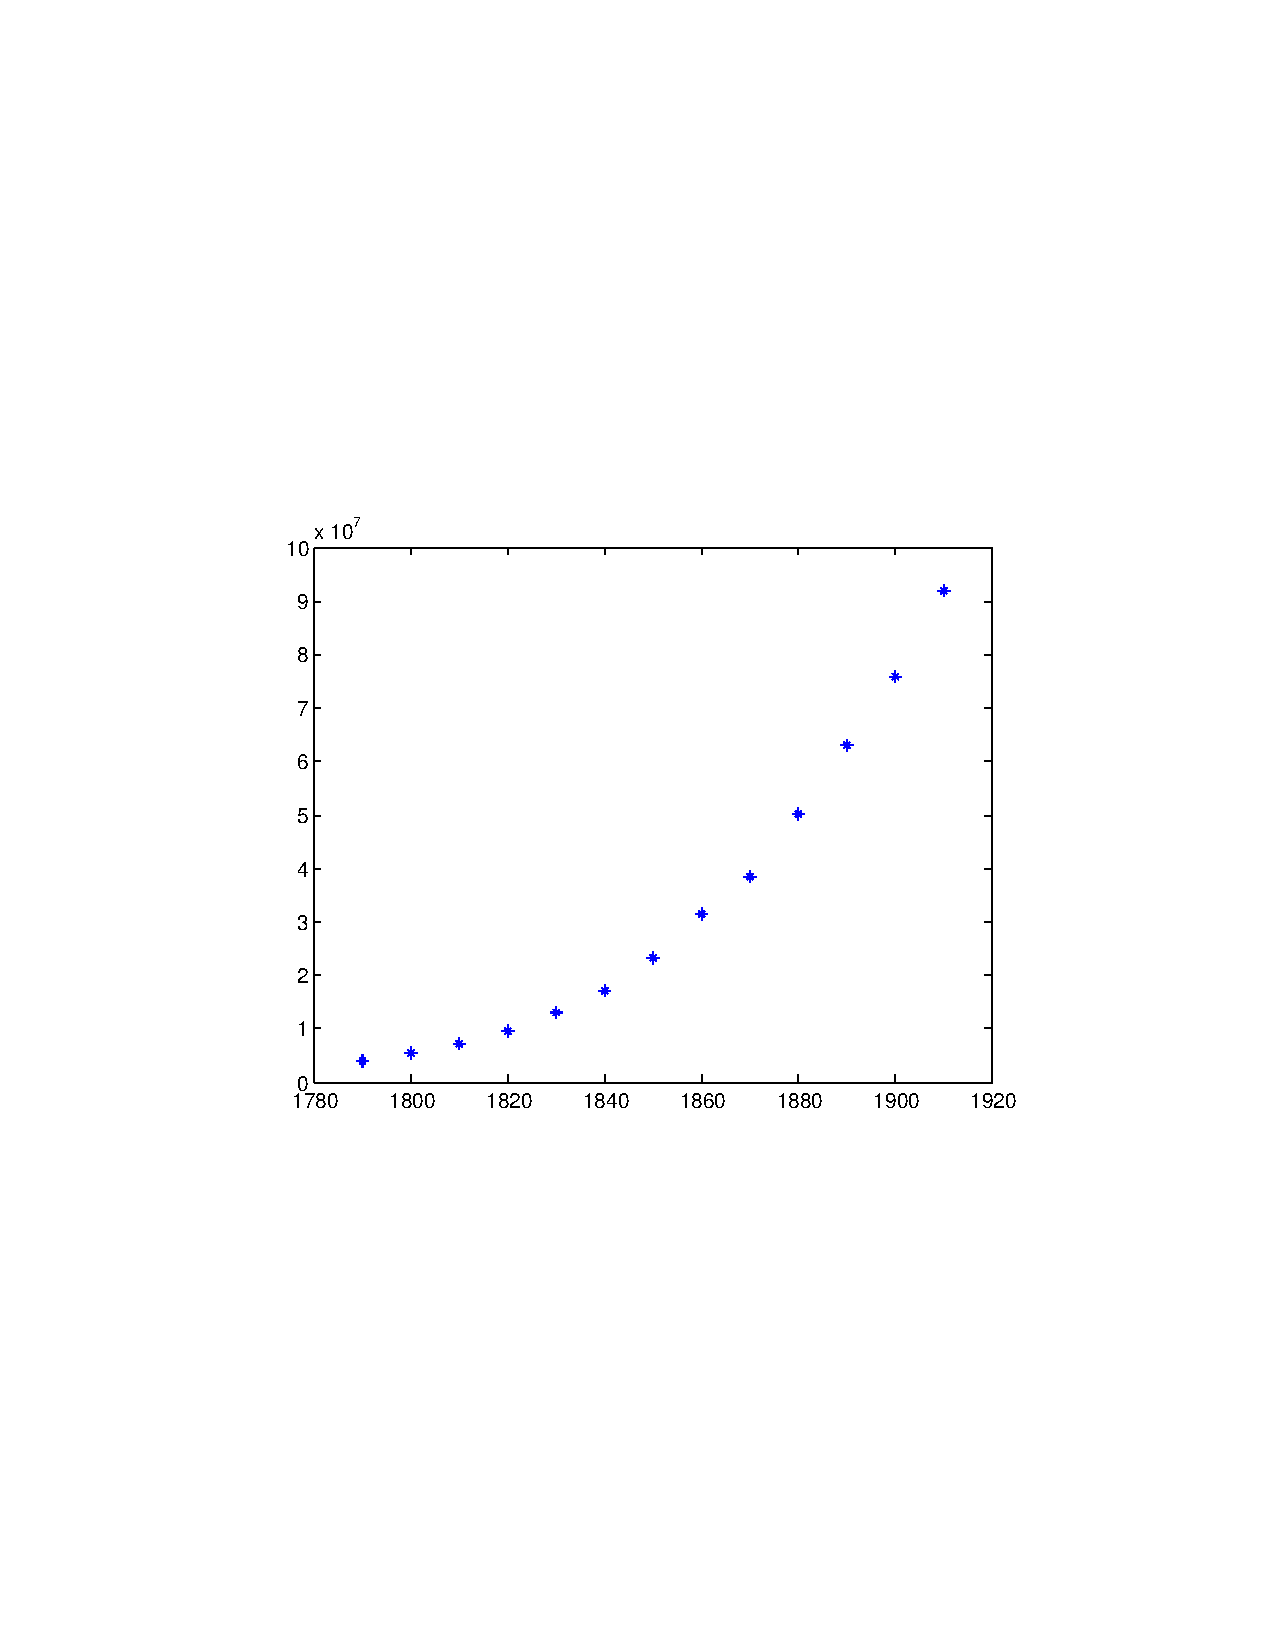
\includegraphics[width=0.9\textwidth]{USpop_to1910_points}
\end{center}
}

\section{A quadratic curve?}

\frame{\frametitle{First idea}
The curve looks like a piece of a parabola. So let us fit a curve of the form
\[
P(t)=a+bt+ct^2.
\]
To do this, we want to minimize
\[
S=\sum_{k=1}^{13} \left(P(t_k)-P_k\right)^2,
\]
where $t_k$ are the known dates, $P_k$ are the known populations, and $P(t_k)=a+bt_k+ct_k^2$.
}

\frame{ 
We proceed as in the notes (but note that the role of $a,b,c$ is reversed):
\[
S=S(a,b,c)=\sum_{k=1}^{13} \left(a+bt_k+ct_k^2-P_k\right)^2
\]
is maximal if (necessary condition) $\partial S/\partial a=\partial S/\partial b=\partial S/\partial c=0$, with
\begin{align*}
\frac{\partial S}{\partial a} &= 2\sum_{k=1}^{13}(a+bt_k+ct_k^2-P_k) \\
\frac{\partial S}{\partial b} &= 2\sum_{k=1}^{13}(a+bt_k+ct_k^2-P_k)t_k \\
\frac{\partial S}{\partial c} &= 2\sum_{k=1}^{13}(a+bt_k+ct_k^2-P_k)t_k^2
\end{align*}
}

\frame{
So we want
\begin{align*}
2\sum_{k=1}^{13}(a+bt_k+ct_k^2-P_k) &= 0\\
2\sum_{k=1}^{13}(a+bt_k+ct_k^2-P_k)t_k &= 0 \\
2\sum_{k=1}^{13}(a+bt_k+ct_k^2-P_k)t_k^2 &= 0,
\end{align*}
that is
\begin{align*}
\sum_{k=1}^{13}(a+bt_k+ct_k^2-P_k) &= 0\\
\sum_{k=1}^{13}(a+bt_k+ct_k^2-P_k)t_k &= 0 \\
\sum_{k=1}^{13}(a+bt_k+ct_k^2-P_k)t_k^2 &= 0.
\end{align*}
}

\frame{
Rearranging the system
\begin{align*}
\sum_{k=1}^{13}(a+bt_k+ct_k^2-P_k) &= 0\\
\sum_{k=1}^{13}(a+bt_k+ct_k^2-P_k)t_k &= 0 \\
\sum_{k=1}^{13}(a+bt_k+ct_k^2-P_k)t_k^2 &= 0,
\end{align*}
we get
\begin{align*}
\sum_{k=1}^{13}(a+bt_k+ct_k^2) &= \sum_{k=1}^{13}P_k\\
\sum_{k=1}^{13}(at_k+bt_k^2+ct_k^3) &= \sum_{k=1}^{13}P_kt_k\\
\sum_{k=1}^{13}(at_k^2+bt_k^3+ct_k^4) &= \sum_{k=1}^{13}P_kt_k^2.
\end{align*}
}

\frame{
\begin{align*}
\sum_{k=1}^{13}(a+bt_k+ct_k^2) &= \sum_{k=1}^{13}P_k\\
\sum_{k=1}^{13}(at_k+bt_k^2+ct_k^3) &= \sum_{k=1}^{13}P_kt_k\\
\sum_{k=1}^{13}(at_k^2+bt_k^3+ct_k^4) &= \sum_{k=1}^{13}P_kt_k^2,
\end{align*}
after a bit of tidying up, takes the form
\begin{align*}
\left(\sum_{k=1}^{13}1\right)a+\left(\sum_{k=1}^{13}t_k\right)b+\left(\sum_{k=1}^{13}t_k^2\right)c &= \sum_{k=1}^{13}P_k \\
\left(\sum_{k=1}^{13}t_k\right)a+\left(\sum_{k=1}^{13}t_k^2\right)b+\left(\sum_{k=1}^{13}t_k^3\right)c &= \sum_{k=1}^{13}P_kt_k \\
\left(\sum_{k=1}^{13}t_k^2\right)a+\left(\sum_{k=1}^{13}t_k^3\right)b+\left(\sum_{k=1}^{13}t_k^4\right)c &= \sum_{k=1}^{13}P_kt_k^2.
\end{align*}
}

\frame{
So the aim is to solve the linear system
\[
\begin{pmatrix}
13 & \sum\limits_{k=1}^{13}t_k & \sum\limits_{k=1}^{13}t_k^2 \\
\sum\limits_{k=1}^{13}t_k & \sum\limits_{k=1}^{13}t_k^2 & \sum\limits_{k=1}^{13}t_k^3 \\
\sum\limits_{k=1}^{13}t_k^2 & \sum\limits_{k=1}^{13}t_k^3 & \sum\limits_{k=1}^{13}t_k^4
\end{pmatrix}
\begin{pmatrix}
a\\ b\\ c
\end{pmatrix}
=
\begin{pmatrix}
\sum\limits_{k=1}^{13}P_k \\
\sum\limits_{k=1}^{13}P_kt_k \\
\sum\limits_{k=1}^{13}P_kt_k^2
\end{pmatrix}
\]
}

\frame[containsverbatim]{
With MatLab (or Octave), getting the values is easy.
\begin{itemize}
\item To apply an operation to every element in a vector or matrix, prefix the operation with a dot, hence
\begin{verbatim}
 t.^2;
\end{verbatim}
gives, for example, the vector with every element $t_k$ squared. 
\item Also, the function {\tt sum} gives the sum of the entries of a vector or matrix.
\item When entering a matrix or vector, separate entries on the same row by {\tt ,} and create a new row by using {\tt ;}.
\end{itemize}
}

\frame[containsverbatim]{
Thus, to set up the problem in the form of solving $Ax=b$, we need to do the following:
\begin{verbatim}
format long g;
A=[13,sum(t),sum(t.^2);sum(t),sum(t.^2),sum(t.^3);...
sum(t.^2),sum(t.^3),sum(t.^4)];
b=[sum(P);sum(P.*t);sum(P.*(t.^2))];
\end{verbatim}
The {\tt format long g} command is used to force the display of digits (normally, what is shown is in ``scientific'' notation, not very informative here). 
}

\frame[containsverbatim]{
Then, solve the system using
\begin{verbatim}
A\b
\end{verbatim}
We get the following output:
\begin{verbatim}
>> A\b
Warning: Matrix is close to singular or badly scaled.
         Results may be inaccurate. RCOND = 1.118391e-020.

ans = 

        22233186177.8195
        -24720291.325476
        6872.99686313725
\end{verbatim}
(note that here, Octave gives a solution that is not as good as this one, provided by MatLab).
}

\section{Checking our results for the quadratic}

\frame[containsverbatim]{
Thus
\[
P(t)=22233186177.8195-24720291.325476t+6872.99686313725t^2
\]
To see what this looks like,
\begin{verbatim}
plot(t,22233186177.8195-24720291.325476.*t...
+6872.99686313725.*t.^2);
\end{verbatim}
(note the dots before multiplication and power, since we apply this function to every entry of $t$).
In fact, to compare with original data:
\begin{verbatim}
plot(t,22233186177.8195-24720291.325476.*t...
+6872.99686313725.*t.^2,t,P,'*');
\end{verbatim}
}

\frame{\frametitle{Our first guess, in pictures}
\begin{center}
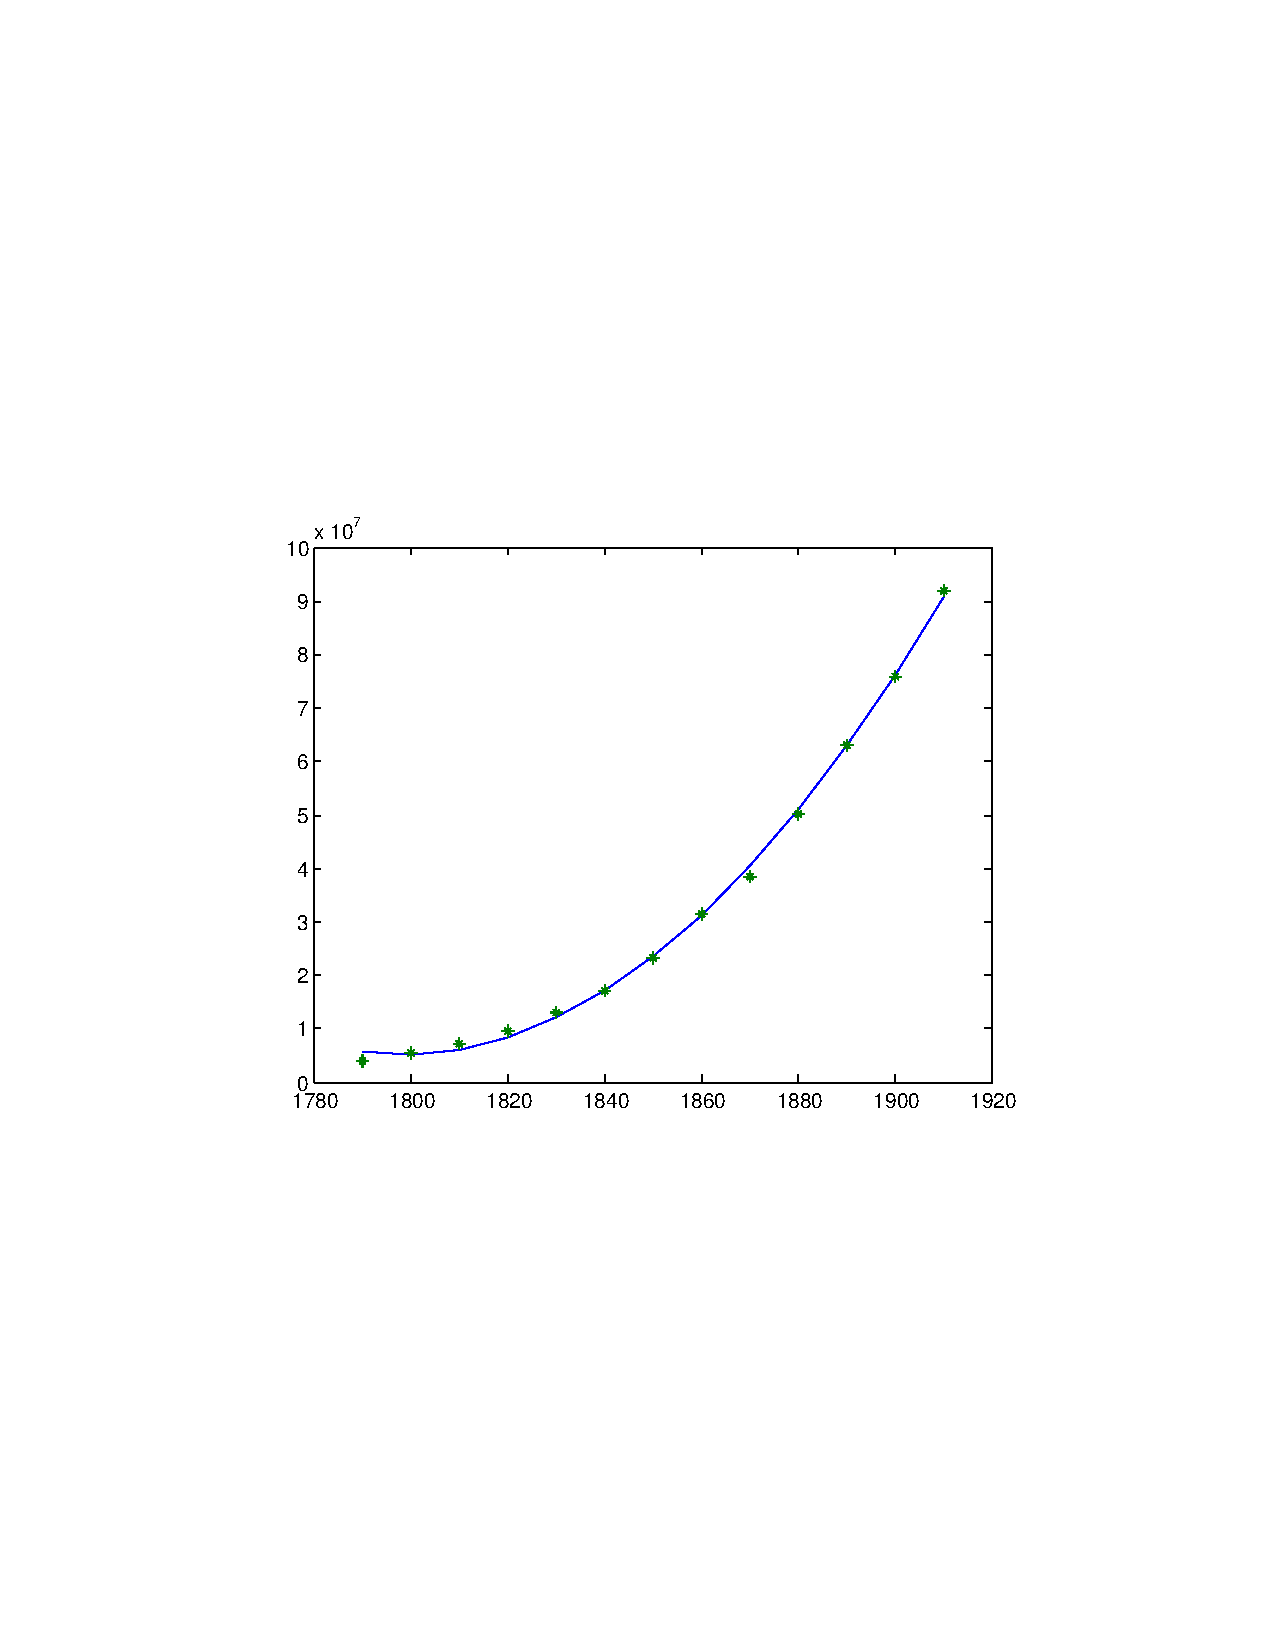
\includegraphics[width=0.9\textwidth]{quadratic_fit}
\end{center}
}


\frame[containsverbatim]{
Now we want to generate the table of values, to compare with the true values and thus compute the error. To do this, we can proceed directly:
\begin{verbatim}
computedP=22233186177.8195-24720291.325476.*t...
+6872.99686313725.*t.^2;
\end{verbatim}
We get
{\tiny
\begin{verbatim}
computedP =

 Columns 1 through 4:

      5633954.39552689      5171628.52739334      6083902.03188705      8370774.90901184

 Columns 5 through 8:

      12032247.1587601      17068318.7811356      23478989.7761383      31264260.1437798

 Columns 9 through 12:

       40424129.884037      50958598.9969215      62867667.4824371      76151335.3405762

 Column 13:

      90809602.5713463
\end{verbatim}}
}

\frame[containsverbatim]{
We can also create an \textbf{inline} function
{\footnotesize
\begin{verbatim}
f=inline('22233186177.8195-24720291.325476.*t+6872.99686313725.*t.^2')
f =

     Inline function:
     f(t) = 22233186177.8195-24720291.325476.*t+6872.99686313725.*t.^2
\end{verbatim}}
This function can then easily be used for a single value
\begin{verbatim}
octave:24> f(1880)
ans =     50958598.9969215
\end{verbatim}
as well as for vectors..
}

\frame[containsverbatim]{
(Recall that $t$ has the dates; $t$ in the definition of the function is a dummy variable, we could have used another letter-.)
\begin{verbatim}
octave:25> f(t)
\end{verbatim}
{\tiny
\begin{verbatim}
ans =

 Columns 1 through 4:

      5633954.39552689      5171628.52739334      6083902.03188705      8370774.90901184

 Columns 5 through 8:

      12032247.1587601      17068318.7811356      23478989.7761383      31264260.1437798

 Columns 9 through 12:

       40424129.884037      50958598.9969215      62867667.4824371      76151335.3405762
12186176863781.4
 Column 13:

      90809602.5713463
\end{verbatim}}
}

\frame[containsverbatim]{
Form the vector of errors, and compute sum of errors squared:
\begin{verbatim}
octave:26> E=f(t)-P;
octave:27> sum(E.^2)
ans =     12186176863781.4
\end{verbatim}
Quite a large error (12,186,176,863,781.4), which is normal since we have used actual numbers, not thousands or millions of individuals, and we are taking the square of the error.
}

\frame[containsverbatim]{
To present things legibly, one way is to put everything in a matrix..
\begin{verbatim}
M=[P;f(t);E;E./P];
\end{verbatim}
This matrix will have each type of information as a row, so to display it in the form of a table, show its transpose, which is achieved using the function {\tt transpose} or the operator $'$.
}


\frame[containsverbatim]{
\footnotesize
\begin{verbatim}
M'
ans =
 3929214      5633954.39552689      1704740.39552689     0.433862954658842
 5308483      5171628.52739334     -136854.472606659   -0.0257803354756263
 7239881      6083902.03188705     -1155978.96811295    -0.159668227711608
 9638453      8370774.90901184     -1267678.09098816    -0.131522983095748
12866020      12032247.1587601     -833772.841239929   -0.0648042550252471
17069453      17068318.7811356     -1134.21886444092  -6.644728828e-05
23191876      23478989.7761383      287113.776138306    0.0123799289086534
31443321      31264260.1437798     -179060.856220245  -0.00569471832254123
38558371       40424129.884037      1865758.88403702    0.0483879073635403
50155783      50958598.9969215      802815.996921539    0.0160064492846526
62947714      62867667.4824371     -80046.5175628662  -0.00127163502018304
75994575      76151335.3405762      156760.340576172   0.00206278330494212
91972266      90809602.5713463     -1162663.42865372    -0.012641456813228
\end{verbatim}
}

\frame[containsverbatim]{\frametitle{Now for the big question...}
How does our formula do for present times?
\begin{verbatim}
f(2006)
ans =     301468584.066013
\end{verbatim}
Actually, quite well: 301,468,584, compared to the 298,444,215 July 2006 estimate, overestimates the population by 3,024,369, a relative error of approximately 1\%.
}

\frame{\frametitle{The US population from 1790 to 2000 (revised numbers)}
\begin{center}
\begin{tabular}[t]{ccc}
\begin{tabular}{cc}
Year & Population\\
& (millions) \\
\hline
1790 & 3.929 \\
1800 & 5.308 \\
1810 & 7.240 \\
1820 & 9.638 \\
1830 & 12.866 \\
1840 & 17.069 \\
1850 & 23.192 \\
1860 & 31.443 \\
1870 & 38.558 \\
1880 & 50.156 \\
1890 & 62.948
\end{tabular} 
&\quad &
\begin{tabular}{cc}
Year & Population \\
& (millions) \\
\hline
1900 & 76.212 \\
1910 & 92.228 \\
1920 & 106.021 \\
1930 & 123.202 \\
1940 & 132.164 \\
1950 & 151.325 \\
1960 & 179.323 \\
1970 & 203.302 \\
1980 & 226.542 \\
1990 & 248.709 \\
2000 & 281.421
\end{tabular}
\end{tabular}
\end{center}
}

\section{Some similar curves}

\frame{\frametitle{Other similar approaches}
Pritchett, 1891:
\[
P=a+bt+ct^2+dt^3.
\]
(we have done this one, and found it to be quite good too).\\
Pearl, 1907:
\[
P(t)=a+bt+ct^2+d\ln t.
\]
Finds
\[
P(t)=9,064,900-6,281,430t+842,377t^2+19,829,500\ln t.
\]
}

\frame{
\begin{center}
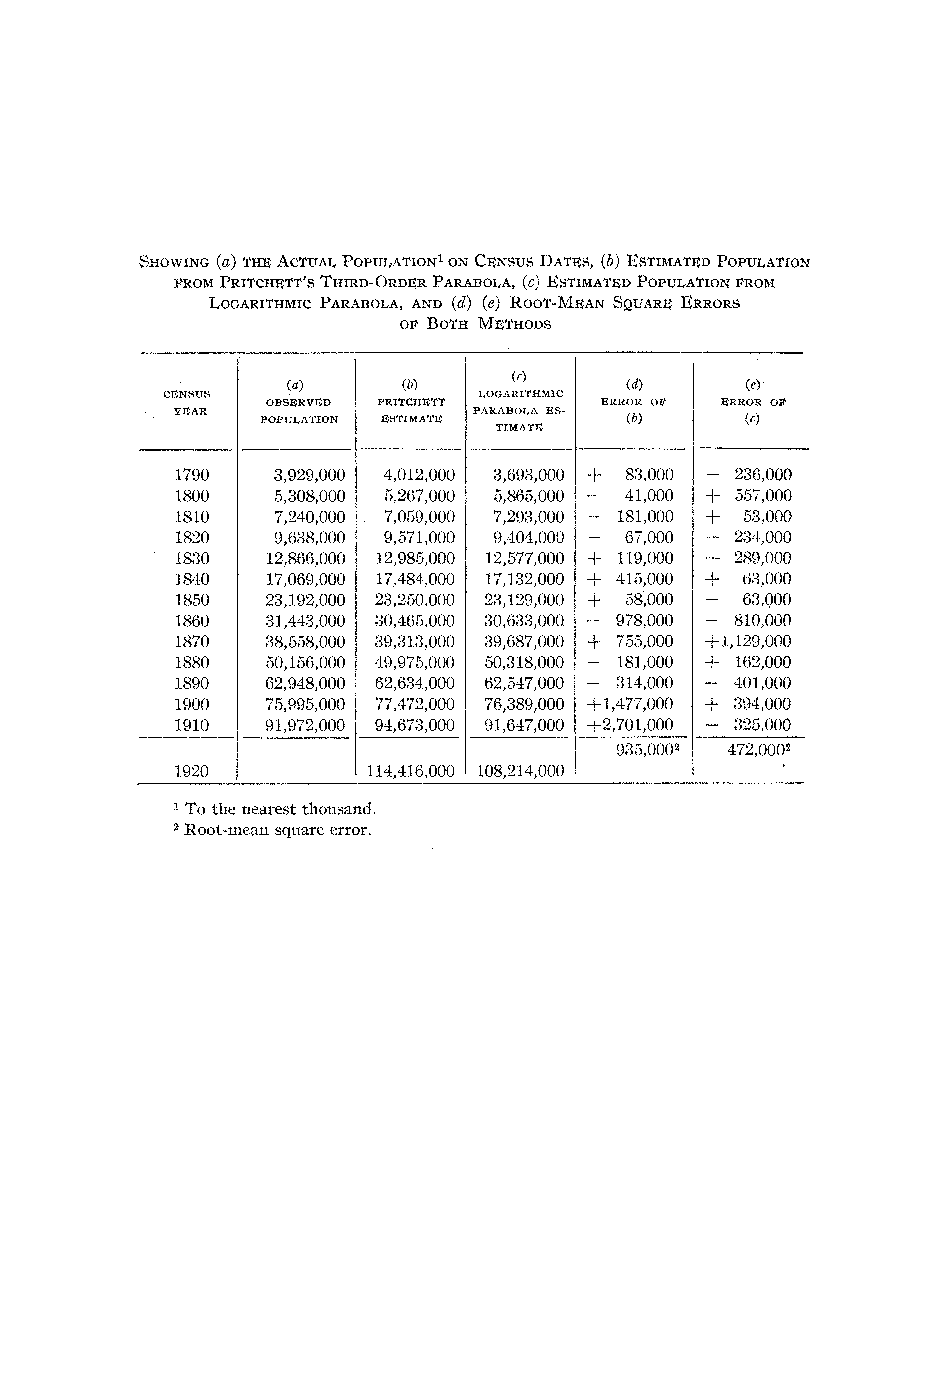
\includegraphics[width=0.95\textwidth]{table2_PearlReed1920PNAS6}
\end{center}
}


\section{Population curves -- Logistic curve}

\frame{\frametitle{The logistic curve}
Pearl and Reed try
\[
P(t)=\frac{be^{at}}{1+ce^{at}}
\]
or
\[
P(t)=\frac{b}{e^{-at}+c}.
\]
%They find
%\[
%P(t)=\frac{2,930.3009}{e^{-0.0313395t}+0.014854}.
%\]
}

\section{Population growth -- Logistic equation}

\frame{\frametitle{The logistic equation}
The logistic curve is the solution to the ordinary differential equation
\[
N'=rN\left(1-\frac NK\right),
\]
which is called the \textbf{logistic equation}. $r$ is the \textbf{intrinsic growth rate}, $K$ is the \textbf{carrying capacity}.
\vskip1cm
This equation was introduced by Pierre-Fran\c{c}ois Verhulst (1804-1849), in 1844.
}

\frame{\frametitle{Deriving the logistic equation}
The idea is to represent a population with the following components:
\begin{itemize}
\item birth, at the \textbf{per capita} rate $b$,
\item death, at the \textbf{per capita} rate $d$,
\item competition of individuals with other individuals reduces their ability to survive, resulting in death.
\end{itemize}
This gives
\[
N'=bN-dN-\textrm{competition}.
\]
}

\frame{\frametitle{Accounting for competition}
Competition describes the mortality that occurs when two individuals meet.
\begin{itemize}
\item
In chemistry, if there is a concentration $X$ of one product and $Y$ of another product, then $XY$, called \textbf{mass action}, describes the number of interactions of molecules of the two products.
\item
Here, we assume that $X$ and $Y$ are of the same type (individuals). So there are $N^2$ contacts.
\item 
These $N^2$ contacts lead to death of one of the individuals at the rate $c$.
\end{itemize}
Therefore, the \textbf{logistic} equation is
\[
N'=bN-dN-cN^2.
\]
}

\frame{\frametitle{Reinterpreting the logistic equation}
The equation
\[
N'=bN-dN-cN^2
\]
is rewritten as
\[
N'=(b-d)N-cN^2.
\]
\begin{itemize}
\item $b-d$ represents the rate at which the population increases (or decreases) in the absence of competition. It is called the \textbf{intrinsic growth rate} of the population.
\item $c$ is the rate of \textbf{intraspecific} competition. The prefix \textbf{intra} refers to the fact that the competition is occurring between members of the same species, that is, within the species.\newline
[We will see later examples of \textbf{interspecific} competition, that is, between different species.]
\end{itemize}
}


\frame{\frametitle{Another (..) interpretation of the logistic equation}
We have
\[
N'=(b-d)N-cN^2.
\]
Factor out an $N$:
\[
N'=\bigl((b-d)-cN\bigr)N.
\]
This gives us another interpretation of the logistic equation. Writing
\[
\frac{N'}N=(b-d)-cN,
\]
we have $N'/N$, the \textbf{per capita growth rate} of $N$, given by a constant, $b-d$, minus a \textbf{density dependent inhibition} factor, $cN$.
}

\frame{\frametitle{Equivalent equations}
\begin{align*}
N' &= (b-d)N-cN^2\\
&= \bigl((b-d)-cN\bigr)N \\
&= \left(r-\frac rr cN\right)N,\quad\textrm{with }r=b-d \\
&= rN\left(1-\frac crN\right) \\
&= rN\left(1-\frac NK\right),
\end{align*}
with
\[
\frac cr=\frac 1K,
\]
that is, $K=r/c$.
}

\frame{\frametitle{3 ways to tackle this equation}
\begin{enumerate}
\item The equation is separable. [explicit method]
\item The equation is a Bernoulli equation. [explicit method]
\item Use qualitative analysis.
\end{enumerate}
}


\section{Qualitative analysis of the logistic equation}

\frame{\frametitle{Studying the logistic equation qualitatively}
We study
\begin{equation}\label{eq:logistic_ode}
N'=rN\left(1-\frac NK\right).\tag{ODE1}
\end{equation}
For this, write
\[
f(N)=rN\left(1-\frac NK\right).
\]
Consider the initial value problem (IVP) 
\begin{equation}\label{ivp:logistic_ode}
N'=f(N),\quad N(0)=N_0>0.\tag{IVP1}
\end{equation}
\begin{itemize}
\item $f$ is $C^1$ (differentiable with continuous derivative) so solutions to \eqref{ivp:logistic_ode} exist and are unique.
\end{itemize}
}

\frame{
\textbf{Equilibria} of \eqref{eq:logistic_ode} are points such that $f(N)=0$ (so that $N'=f(N)=0$, meaning $N$ does not vary). So we solve $f(N)=0$ for $N$. We find two points:
\begin{itemize}
\item $N=0$
\item $N=K$.
\end{itemize}
By uniqueness of solutions to \eqref{ivp:logistic_ode}, solutions cannot cross the lines $N(t)=0$ and $N(t)=K$.
}

\frame{
There are several cases.
\begin{itemize}
\item $N=0$ for some $t$, then $N(t)=0$ for all $t\geq 0$, by uniqueness of solutions.
\item $N\in(0,K)$, then $rN>0$ and $N/K<1$ so $1-N/K>0$, which implies that $f(N)>0$. As a consequence, $N(t)$ increases if $N\in(0,K)$.
\item $N=K$, then $rN>0$ but $N/K=1$ so $1-N/K=0$, which implies that $f(N)=0$. As a consequence, $N(t)=K$ for all $t\geq 0$, by uniqueness of solutions.
\item $N>K$, the $rN>0$ and $N/K>1$, implying that $1-N/K<0$ and in turn, $f(N)<0$. As a consequence, $N(t)$ decreases if $N\in(K,+\infty)$.
\end{itemize}
}

\frame{
Therefore,
\begin{theorem}
Suppose that $N_0>0$. Then the solution $N(t)$ of \eqref{ivp:logistic_ode} is such that
\[
\lim_{t\to\infty} N(t)=K,
\]
so that $K$ is the number of individuals that the environment can support, the \textbf{carrying capacity} of the environment.

If $N_0=0$, then $N(t)=0$ for all $t\geq 0$.
\end{theorem}
}


\section{The delayed logistic equation}
\frame{\frametitle{The delayed logistic equation}
Consider the equation as
\[
\frac{N'}{N}=(b-d)-cN,
\]
that is, the per capita rate of growth of the population depends on the net growth rate $b-d$, and some density dependent inhibition $cN$ (resulting of competition).
\vskip0.5cm
Suppose that instead of instantaneous inhibition, there is some delay $\tau$ between the time the inhibiting event takes place and the moment when it affects the growth rate.
\vskip0.5cm
For example, two individuals fight for food, and one later dies of the injuries sustained during this fight.
}

\frame{\frametitle{The delayed logistic equation}
In the case of a time $\tau$ between inhibiting event and inhibition, the equation would be written as
\[
\frac{N'}N=(b-d)-cN(t-\tau).
\]
Using the change of variables introduced earlier, this is written
\begin{equation}\label{eq:logistic_dde}
N'(t)=rN(t)\left(1-\frac{N(t-\tau)}K\right). \tag{DDE1}
\end{equation}
Such an equation is called a \textbf{delay} differential equation. It is much more complicated to study than \eqref{eq:logistic_ode}. In fact, some things remain unknown about \eqref{eq:logistic_dde}.
}

\frame{\frametitle{Delayed initial value problem}
The IVP takes the form
\begin{equation}\label{ivp:logistic_dde}
\begin{aligned}
N'(t)&= rN(t)\left(1-\frac{N(t-\tau)}K\right),\\
N(t) &= \phi(t)\textrm{ for }t\in[-\tau,0],
\end{aligned} \tag{IVP2}
\end{equation}
where $\phi(t)$ is some continuous function. Hence, initial conditions (called initial data in this case) must be specified on an interval, instead of being specified at a point, to guarantee existence and uniqueness of solutions.

We will not learn how to study this type of equation (this is graduate level mathematics). I will give a few results.
}

\frame{
To find equilibria, remark that delay should not play a role, since $N$ should be constant. Thus, equilibria are found by considering the equation with no delay, which is \eqref{eq:logistic_ode}.
\begin{theorem}
Suppose that $r\tau<\pi/2$. Then solutions of \eqref{ivp:logistic_dde} with positive initial data $\phi(t)$ starting close enough to $K$ tend to $K$. If $r\tau<37/24$, then all solutions of  \eqref{ivp:logistic_dde} with positive initial data $\phi(t)$ tend to $K$. If $r\tau>\pi/2$, then $K$ is an unstable equilibrium and all solutions of \eqref{ivp:logistic_dde} with positive initial data $\phi(t)$ on $[-\tau,0]$ are oscillatory.
\end{theorem}
\vskip1cm

There is a gray zone between $37/24$ ($\simeq 1.5417$) and $\pi/2$ ($\simeq 1.5708$). The global aspect was proved for $r\tau<37/24$ in 1945 by Wright. Although there is very strong numerical evidence that this is in fact true up to $\pi/2$, nobody has yet managed to prove it.
}

\section{The logistic map}

\frame{\frametitle{Discrete-time systems}
So far, we have seen continuous-time models, where $t\in\IR_+$. Another way to model natural phenomena is by using a discrete-time formalism, that is, to consider equations of the form
\[
x_{t+1}=f(x_t),
\]
where $t\in\IN$ or $\IZ$, that is, $t$ takes values in a discrete valued (countable) set.
\vskip0.5cm
Time could for example be days, years, etc.
}


\frame{\frametitle{The logistic map}
The logistic \textbf{map} is, for $t\geq 0$,
\begin{equation}\label{eq:logistic_discrete}
N_{t+1}=rN_t\left(1-\frac{N_t}K\right). \tag{DT1}
\end{equation}
To transform this into an initial value problem, we need to provide an initial condition $N_0\geq 0$ for $t=0$.
}


\frame{\frametitle{Some mathematical analysis}
Suppose we have a system in the form
\[
x_{t+1}=f(x_t),
\]
with initial condition given for $t=0$ by $x_0$. Then,
\begin{align*}
x_1 &= f(x_0) \\
x_2 &= f(x_1)= f(f(x_0))\stackrel{\Delta}{=} f^2(x_0) \\
& \vdots \\
x_k &= f^k(x_0).
\end{align*}
The $f^k=\underbrace{f\circ f\circ\cdots\circ f}_{k\textrm{ times}}$ are called the \textbf{iterates} of $f$.
}

\frame{\frametitle{Fixed points}
\begin{definition}[Fixed point]
Let $f$ be a function. A point $p$ such that $f(p)=p$ is called a \textbf{fixed point} of $f$.
\end{definition}
\begin{theorem}
Consider the closed interval $I=[a,b]$. If $f:I\to I$ is continuous, then $f$ has a fixed point in $I$.
\end{theorem}
\begin{theorem}
Let $I$ be a closed interval and $f:I\to\IR$ be a continuous function. If $f(I)\supset I$, then $f$ has a fixed point in $I$.
\end{theorem}
}

\frame{\frametitle{Periodic points}
\begin{definition}[Periodic point]
Let $f$ be a function. If there exists a point $p$ and an integer $n$ such that
\[
f^n(p)=p,\quad\textrm{but}\quad f^k(p)\neq p\textrm{ for }k<n,
\]
then $p$ is a periodic point of $f$ with (least) period $n$ (or a $n$-periodic point of $f$).
\end{definition}
\vskip0.5cm
Thus, $p$ is a $n$-periodic point of $f$ iff $p$ is a $1$-periodic point of $f^n$.
}


\frame{\frametitle{Stability of fixed points, of periodic points}
\begin{theorem}
Let $f$ be a continuously differentiable function (that is, differentiable with continuous derivative, or $C^1$), and $p$ be a fixed point of $f$. 
\begin{enumerate}
\item If $|f'(p)|<1$, then there is an open interval $\mathcal{I}\ni p$ such that $\lim_{k\to\infty}f^k(x)=p$ for all $x\in\mathcal{I}$.
\item If $|f'(p)|>1$, then there is an open interval $\mathcal{I}\ni p$ such that if $x\in\mathcal{I}$, $x\neq p$, then there exists $k$ such that $f^k(x)\not\in\mathcal{I}$.
\end{enumerate}
\end{theorem}
\begin{definition}
Suppose that $p$ is a $n$-periodic point of $f$, with $f\in C^1$. 
\begin{itemize}
\item If $|\left(f^n\right)'(p)|<1$, then $p$ is an \textbf{attracting} periodic point of $f$. 
\item If $|\left(f^n\right)'(p)|>1$, then $p$ is an \textbf{repelling} periodic point of $f$.
\end{itemize}
\end{definition}
}

\frame{\frametitle{Parametrized families of functions}
Consider the equation \eqref{eq:logistic_discrete}, which for convenience we rewrite as
\begin{equation}\label{eq:logistic_discrete_scaled}
N_{t+1}=rN_t(1-N_t)\tag{DT2},
\end{equation}
where $r$ is a parameter in $\IR_+$, and $N$ will typically be taken in $[0,1]$. Let
\[
f_r(x)=rx(1-x).
\]
The function $f_r$ is called a \textbf{parametrized family} of functions.
}

\frame{\frametitle{Bifurcations}
\begin{definition}[Bifurcation]
Let $f_\mu$ be a parametrized family of functions. Then there is a \textbf{bifurcation} at $\mu=\mu_0$ (or $\mu_0$ is a bifurcation point) if there exists $\varepsilon>0$ such that, if $\mu_0-\varepsilon<a<\mu_0$ and $\mu_0<b<\mu_0+\varepsilon$, then the dynamics of $f_a(x)$ are ``different'' from the dynamics of $f_b(x)$.
\end{definition}
\vskip0.5cm
An example of ``different'' would be that $f_a$ has a fixed point (that is, a 1-periodic point) and $f_b$ has a 2-periodic point.
}


\frame{\frametitle{Back to the logistic map}
Consider the simplified version \eqref{eq:logistic_discrete_scaled},
\[
N_{t+1}=rN_t(1-N_t)\stackrel{\Delta}{=}f_r(N_t).
\]
{\bf Are solutions well defined?}
Suppose $N_0\in[0,1]$, do we stay in $[0,1]$? 
$f_r$ is continuous on $[0,1]$, so it has a extrema on $[0,1]$. We have
\[
f_r'(x)=r-2rx=r(1-2x),
\]
which implies that $f_r$ increases for $x<1/2$ and decreases for $x>1/2$, reaching a maximum at $x=1/2$. 
\vskip0.5cm
$f_r(0)=f_r(1)=0$ are the minimum values, and $f(1/2)=r/4$ is the maximum. Thus, if we want $N_{t+1}\in[0,1]$ for $N_t\in[0,1]$, we need to consider $r\leq 4$.
}

\frame{
\begin{itemize}
\item Note that if $N_0=0$, then $N_t=0$ for all $t\geq 1$. 
\item Similarly, if $N_0=1$, then $N_1=0$, and thus $N_t=0$ for all $t\geq 1$.
\item This is true for all $t$: if there exists $t_k$ such that $N_{t_k}=1$, then $N_t=0$ for all $t\geq t_k$.
\item This last case might occur if $r=4$, as we have seen.
\item Also, if $r=0$ then $N_t=0$ for all $t$.
\end{itemize}
For these reasons, we generally consider
\[
N\in(0,1)
\]
and
\[
r\in(0,4).
\]
}

\frame{\frametitle{Fixed points: existence}
{\bf Fixed points} of \eqref{eq:logistic_discrete_scaled} satisfy $N=rN(1-N)$, giving:
\begin{itemize}
\item $N=0$;
\item $1=r(1-N)$, that is, $p\stackrel{\Delta}{=}\dfrac{r-1}{r}$. 
\end{itemize}
Note that $\lim_{r\to 0^+}p=1-\lim_{r\to 0^+}1/r=-\infty$, $\frac{\partial}{\partial r}p=1/r^2>0$ (so $p$ is an increasing function of $r$), $p=0\Leftrightarrow r=1$ and $\lim_{r\to\infty}p=1$. 
So we come to this first conclusion:
\begin{itemize}
\item 0 always is a fixed point of $f_r$.
\item If $0<r<1$, then $p$ takes negative values so is not relevant.
\item If $1<r<4$, then $p$ exists.
\end{itemize}
}


\frame{\frametitle{Stability of the fixed points}
{\bf Stability} of the fixed points is determined by the (absolute) value $f_r'$ at these fixed points. We have
\[
|f'_r(0)|=r,
\]
and
\begin{align*}
|f'_r(p)| &= \left|r-2r\dfrac{r-1}{r}\right|\\
&= |r-2(r-1)| \\
&= |2-r|
\end{align*}
Therefore, we have
\begin{itemize}
\item if $0<r<1$, then the fixed point $N=p$ does not exist and $N=0$ is attracting,
\item if $1<r<3$, then $N=0$ is repelling, and $N=p$ is attracting,
\item if $r>3$, then $N=0$ and $N=p$ are repelling.
\end{itemize}
}

\frame{
\begin{center}
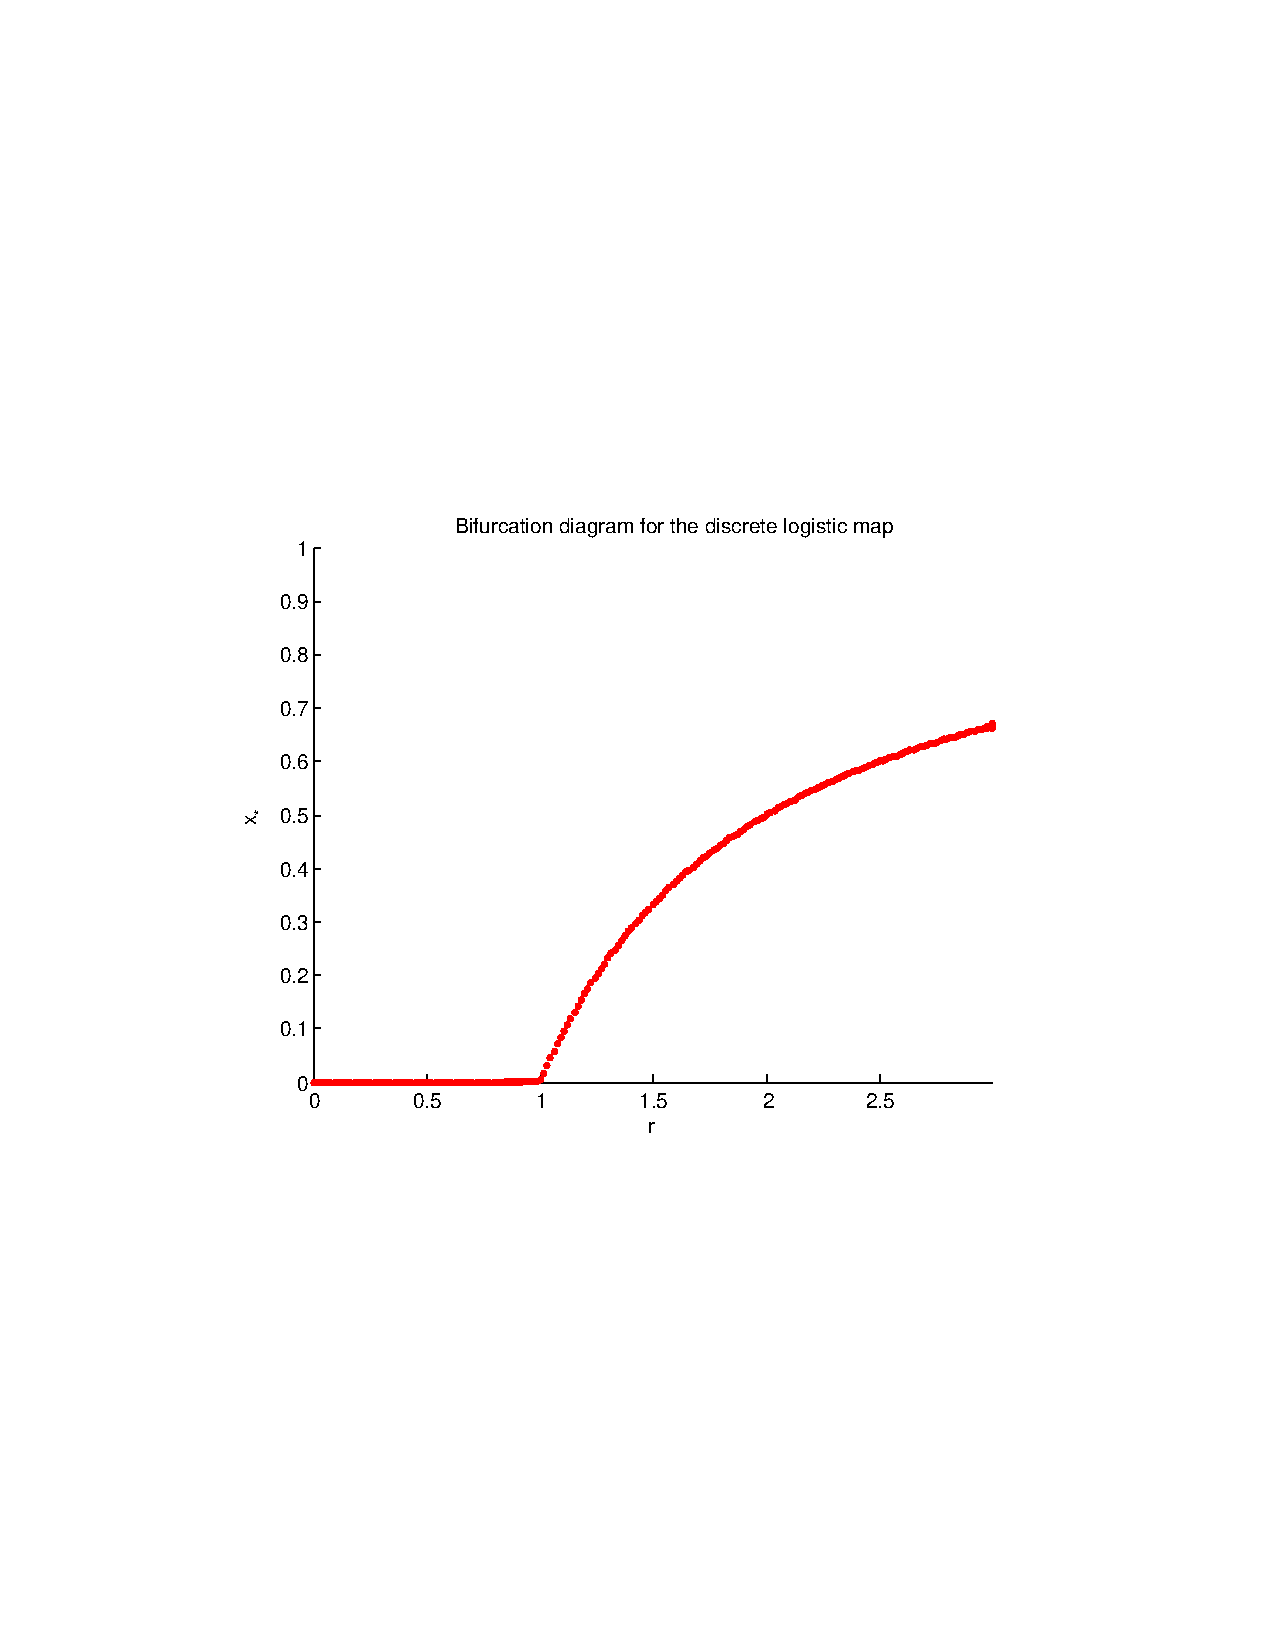
\includegraphics[width=0.9\textwidth]{bif_cascade_1}
\end{center}
}


\frame{\frametitle{Another bifurcation}
Thus the points $r=1$ and $r=3$ are bifurcation points. To see what happens when $r>3$, we need to look for period 2 points.

\begin{align}
f_r^2(x) &= f_r(f_r(x)) \nonumber\\
&= r f_r(x)(1-f_r(x)) \nonumber\\
&= r^2 x(1-x)(1-r x(1-x)). \label{eq:f_mu_2_a}
\end{align}
0 and $p$ are points of period 2, since a fixed point $x^*$ of $f$ satisfies $f(x^*)=x^*$, and so, $f^2(x^*)=f(f(x^*))=f(x^*)=x^*$. 

This helps localizing the other periodic points. Writing the fixed point equation as
\[
Q(x)\stackrel{\Delta}{=}f_r^2(x)-x=0,
\]
we see that, since $0$ and $p$ are fixed points of $f_\mu^2$, they are roots of $Q(x)$. Therefore, $Q$ can be factorized as
\[
Q(x)=x(x-p)(-r^3x^2+Bx+C),
\]
}


\frame{
Substitute the value $(r-1)/r$ for $p$ in $Q$, develop $Q$ and \eqref{eq:f_mu_2_a} and equate coefficients of like powers gives
\begin{equation}\label{eq:Q}
Q(x)=x\left(x-\frac{r-1}{r}\right)\left(-r^3 x^2+r^2(r+1)x-r(r+1)\right).
\end{equation}
We already know that $x=0$ and $x=p$ are roots of \eqref{eq:Q}. So we search for roots of
\[
R(x):=-r^3 x^2+r^2(r+1)x-r(r+1).
\]
Discriminant is 
\begin{align*}
\Delta &=r^4(r+1)^2-4r^4(r+1)\\ 
&= r^4(r+1)(r+1-4)\\
&= r^4(r+1)(r-3). 
\end{align*}
Therefore, $R$ has distinct real roots if $r>3$.
Remark that for $r=3$, the (double) root is $p=2/3$. For $r>3$ but very close to 3, it follows from the continuity of $R$ that the roots are close to $2/3$.

}


\frame{\frametitle{Descartes' rule of signs}
\begin{theorem}[Descartes' rule of signs]\label{th:descartes}
Let $p(x) = \sum_{i=0}^m a_ix^i $ be a polynomial with real coefficients such that $a_m \neq 0$.
Define $v$ to be the number of {\it variations in sign} of the sequence of coefficients $a_m, \ldots, a_0$. By 'variations in sign' we mean the number of values of $n$ such that the sign of $a_n$ differs from the sign of $a_{n - 1}$, as $n$ ranges from $m$ down to 1.
Then 
\begin{itemize}
\item the number of positive real roots of $p(x)$ is $v-2N$ for some integer $N$ satisfying $0 \leq N \leq \dfrac{v}{2}$,
\item the number of negative roots of $p(x)$ may be obtained by the same method by applying the rule of signs to $p(-x)$.
\end{itemize}
\end{theorem}
}

\frame{\frametitle{Example of use of Descartes' rule}
\begin{example}
Let 
\[
p(x) = x^3+3x^2-x-3.
\] 
Coefficients have signs $++--$, i.e., 1 sign change.
Thus $v = 1$. Since $0 \leq N \leq 1/2$, we must have $N=0$. Thus $v-2N=1$ and there is exactly one positive real root of $p(x)$.

To find the negative roots, we examine $p(-x) = -x^3+3x^2+x-3$. Coefficients have signs $-++-$, i.e., 2 sign changes. Thus $v=2$ and $0 \leq N \leq 2/2= 1$.
Thus, there are two possible solutions, $N=0$ and $N=1$, and two possible values of $v-2N$. Therefore, there are either two or no negative real roots.
Furthermore, note that $p(-1)=(-1)^3+3 \cdot (-1)^2-(-1)-3=0$, hence there is at least one negative root. Therefore there must be exactly two.
\end{example}
}

\frame{\frametitle{Back to the logistic map and the polynomial $R$..}
We use Descartes' rule of signs. 
\begin{itemize}
\item
$R$ has signed coefficients $-+-$, so 2 sign changes imlying 0 or 2 positive real roots. 
\item
$R(-x)$ has signed coefficients $---$, so no negative real roots. 
\item 
Since $\Delta>0$, the roots are real, and thus it follows that both roots are positive.
\end{itemize}
To show that the roots are also smaller than 1, consider the change of variables $z=x-1$. The polynomial $R$ is transformed into 
\begin{align*}
R_2(z) &= -r^3 (z+1)^2+r^2(r+1)(z+1)-r(r+1) \\
&= -r^3z^2+r^2(1-r)z-r.
\end{align*}
For $r>1$, the signed coefficients are $---$, so $R_2$ has no root $z>0$, implying in turn that $R$ has no root $x>1$.
}


\frame{\frametitle{Summing up}
\begin{itemize}
\item If $0<r<1$, then $N=0$ is attracting, $p$ does not exist and there are no period 2 points.
\item At $r=1$, there is a bifurcation (called a \textbf{transcritical} bifurcation).
\item If $1<r<3$, then $N=0$ is repelling, $N=p$ is attracting, and there are no period 2 points.
\item At $r=3$, there is another bifurcation (called a \textbf{period-doubling} bifurcation).
\item For $r>3$, both $N=0$ and $N=p$ are repelling, and there is a period 2 point.
\end{itemize}
}

\frame{
\begin{center}
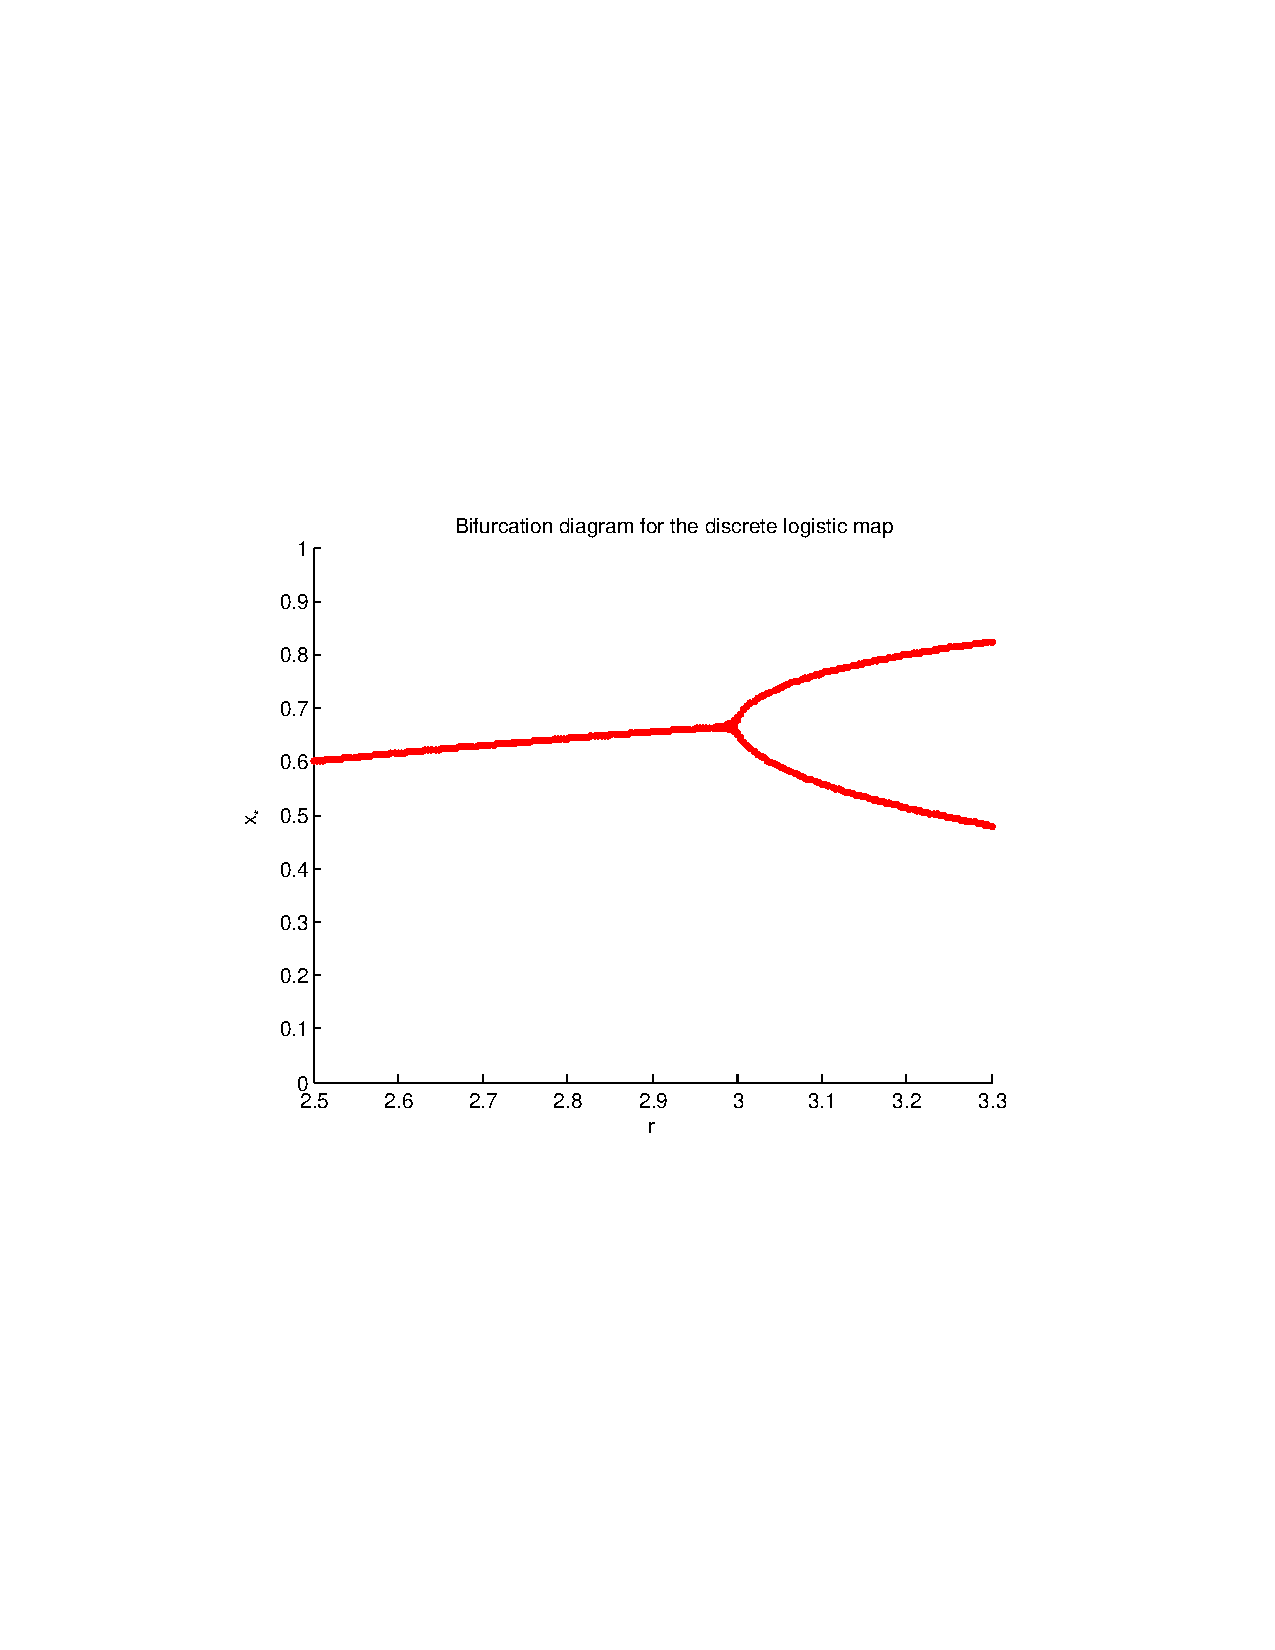
\includegraphics[width=0.9\textwidth]{bif_cascade_2}
\end{center}
}
\frame{
\begin{center}
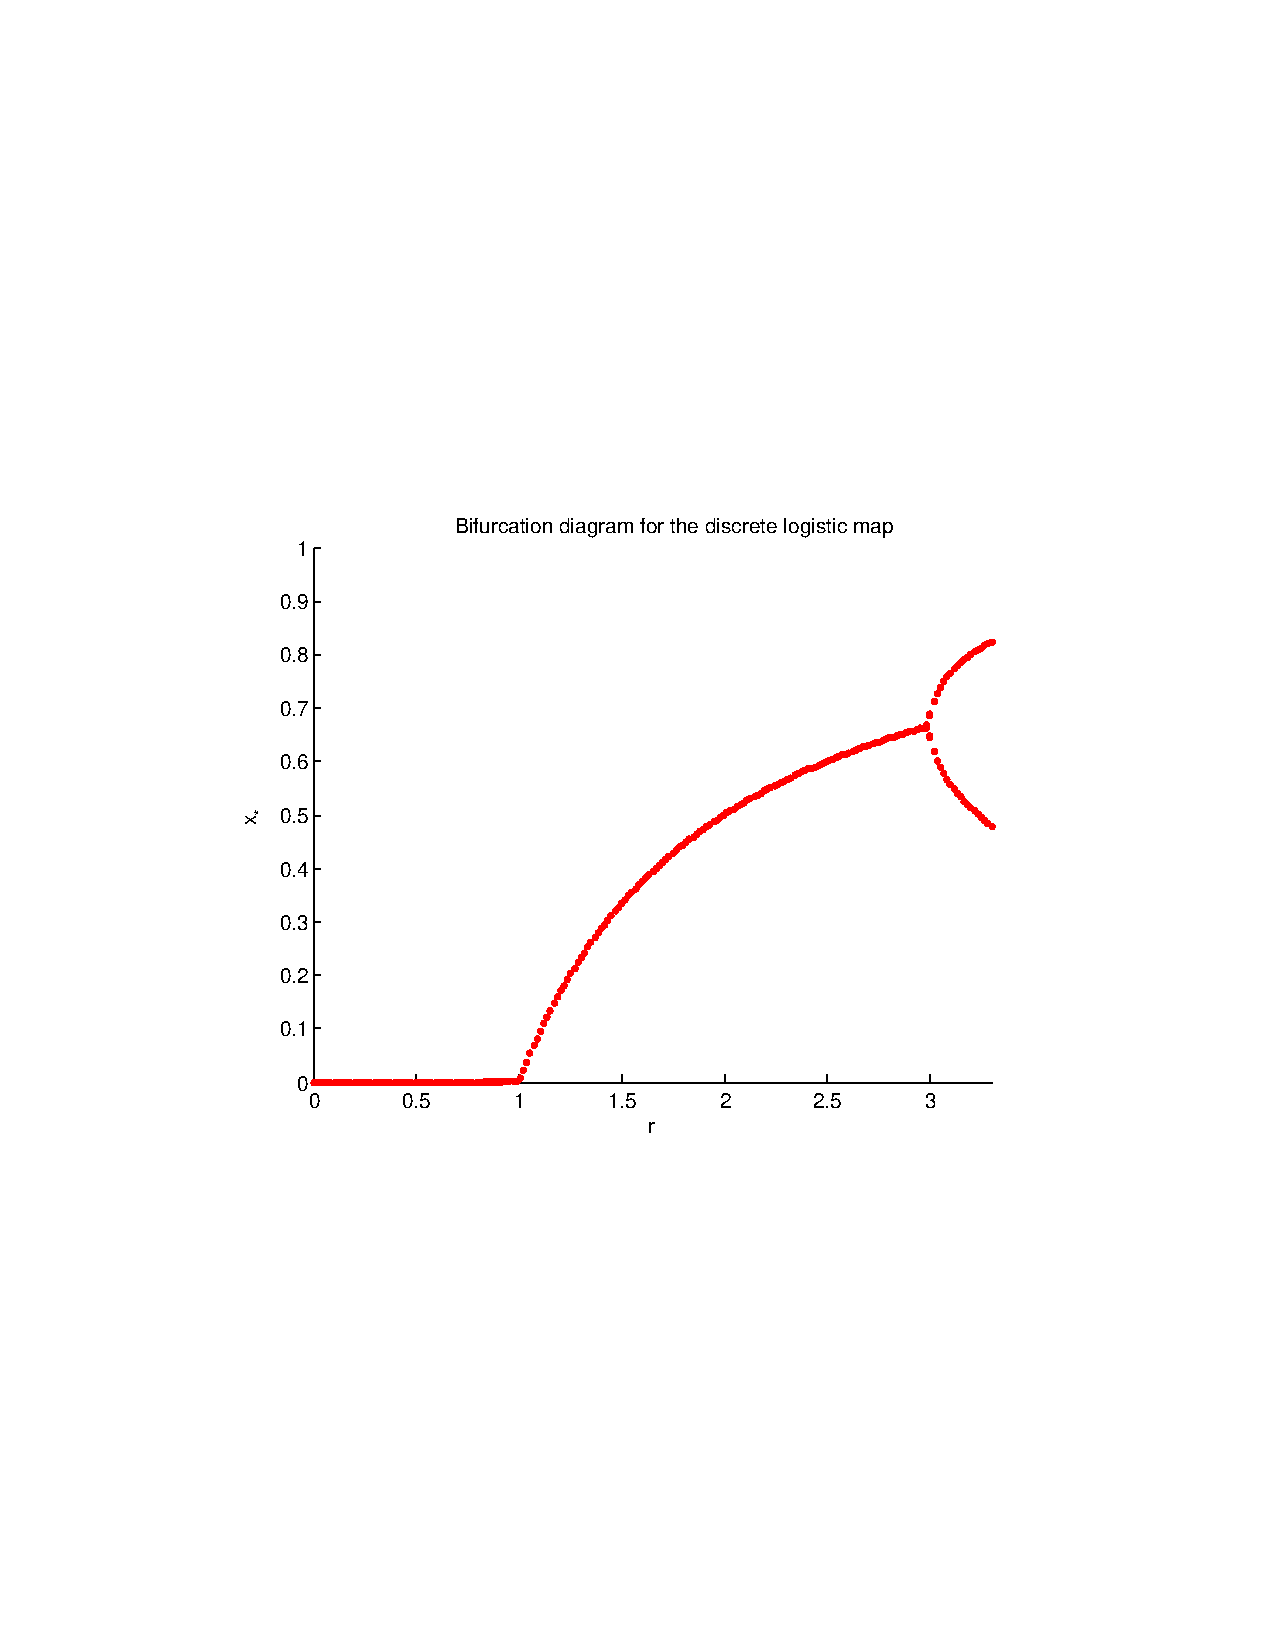
\includegraphics[width=0.9\textwidth]{bif_cascade_3}
\end{center}
}


\frame{\frametitle{This process continues}
\begin{center}
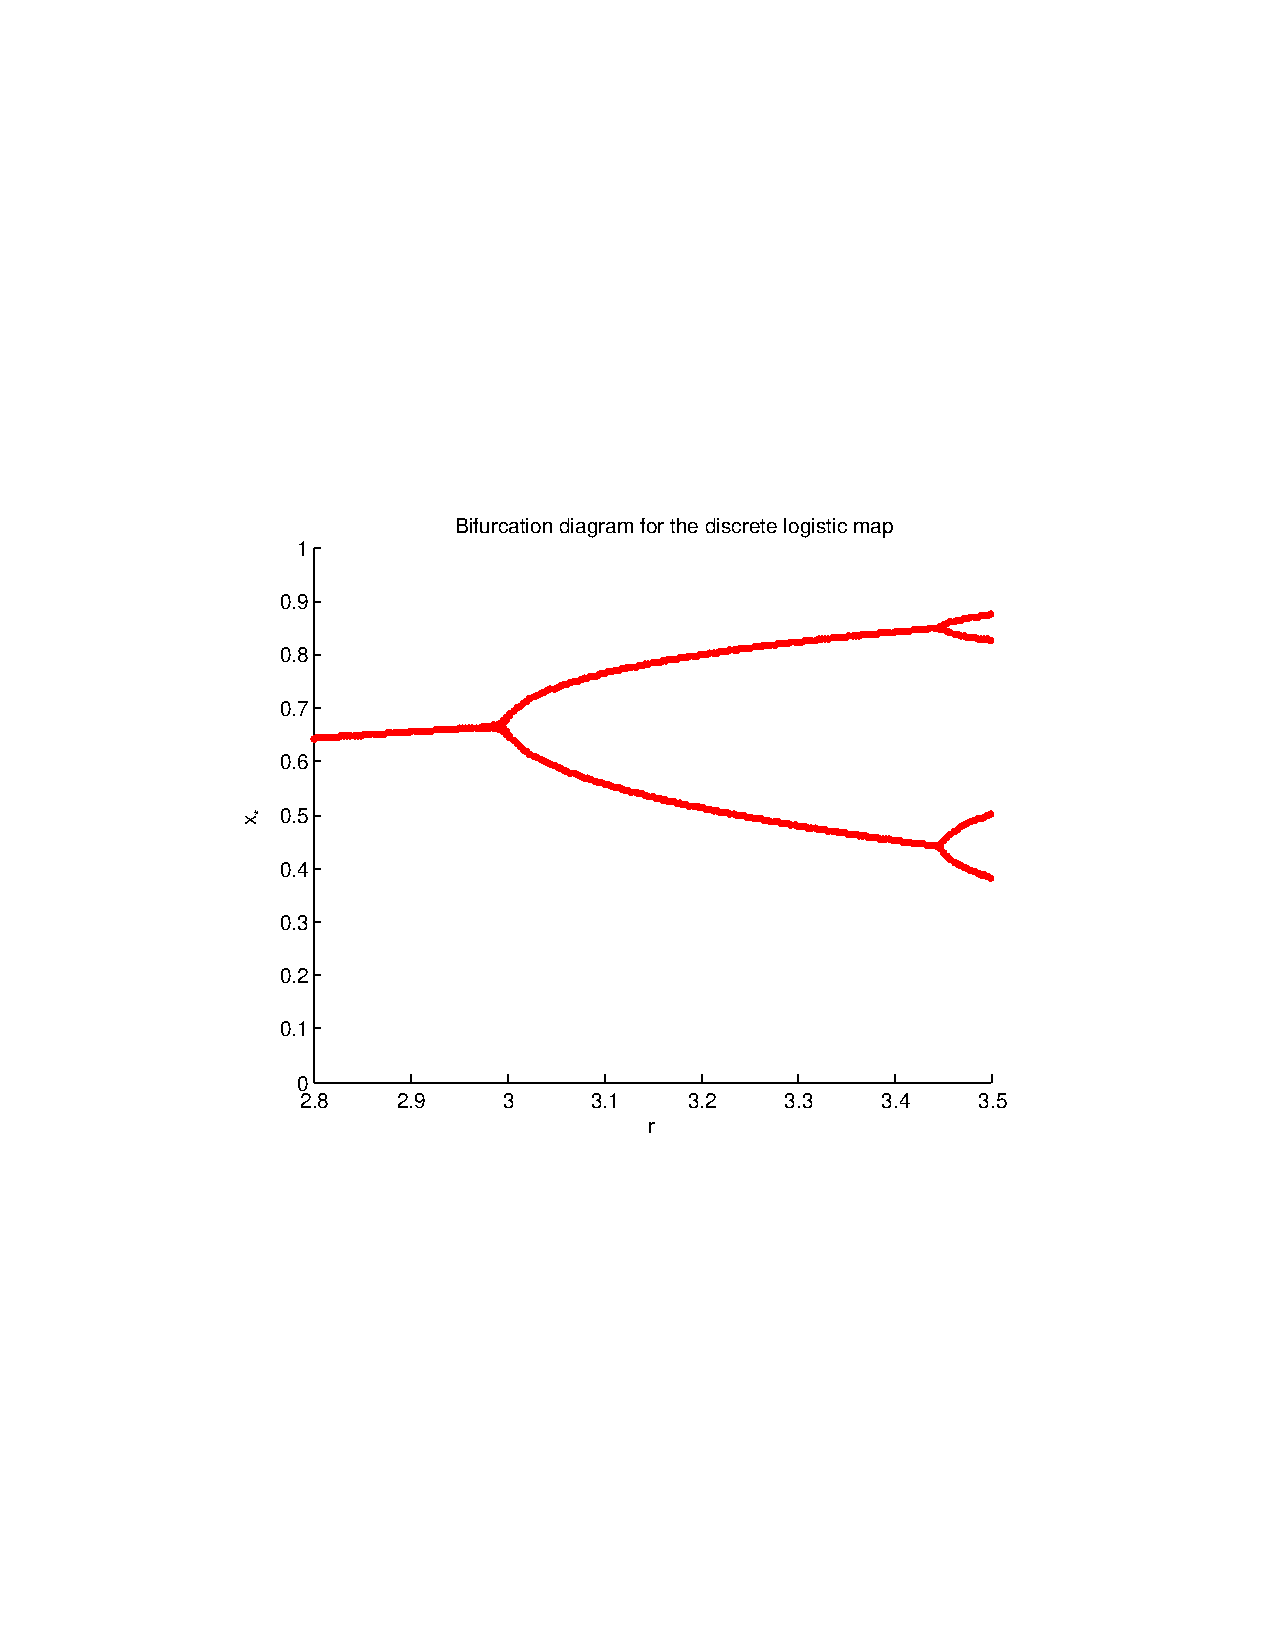
\includegraphics[width=0.9\textwidth]{bif_cascade_4}
\end{center}
}

\frame{\frametitle{The period-doubling cascade to chaos}
The logistic map undergoes a sequence of period doubling bifurcations, called the \textbf{period-doubling cascade}, as $r$ increases from 3 to 4.

\begin{itemize}
\item Every successive bifurcation leads to a doubling of the period.
\item The bifurcation points form a sequence, $\{r_n\}$, that has the property that
\[
\lim{n\to\infty}\frac{r_n-r_{n-1}}{r_{n+1}-r_n}
\]
exists and is a constant, called the Feigenbaum constant, equal to 4.669202\ldots
\item This constant has been shown to exist in many of the maps that undergo the same type of cascade of period doubling bifurcations.
\end{itemize}
}


\frame{\frametitle{Chaos}
After a certain value of $r$, there are periodic points with all periods. In particular, there are periodic points of period 3. 
\vskip1cm
By a theorem (called \textbf{Sarkovskii's theorem}), the presence of period 3 points implies the presence of points of all periods.
\vskip1cm
At this point, the system is said to be in a \textbf{chaotic regime}, or \textbf{chaotic}.
}

\frame{\frametitle{Bifurcation cascade for $2.9\leq r\leq 4$}
\begin{center}
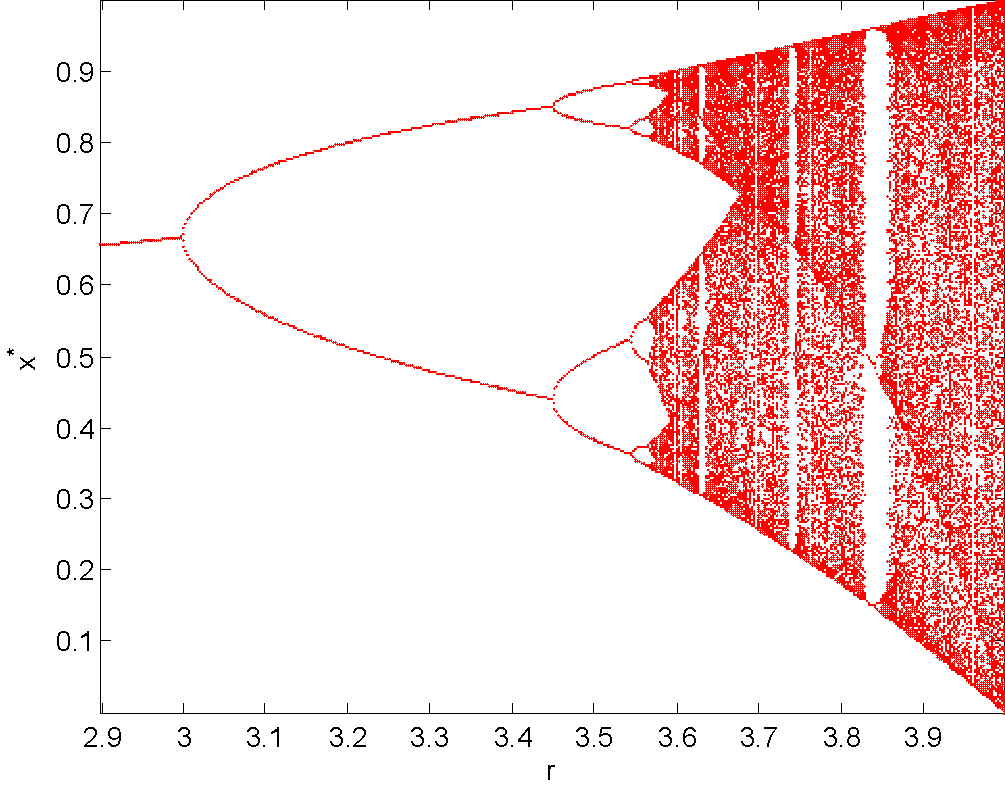
\includegraphics[width=0.9\textwidth]{cascade_29_4}
\end{center}
}

\frame{\frametitle{The complete bifurcation cascade}
\begin{center}
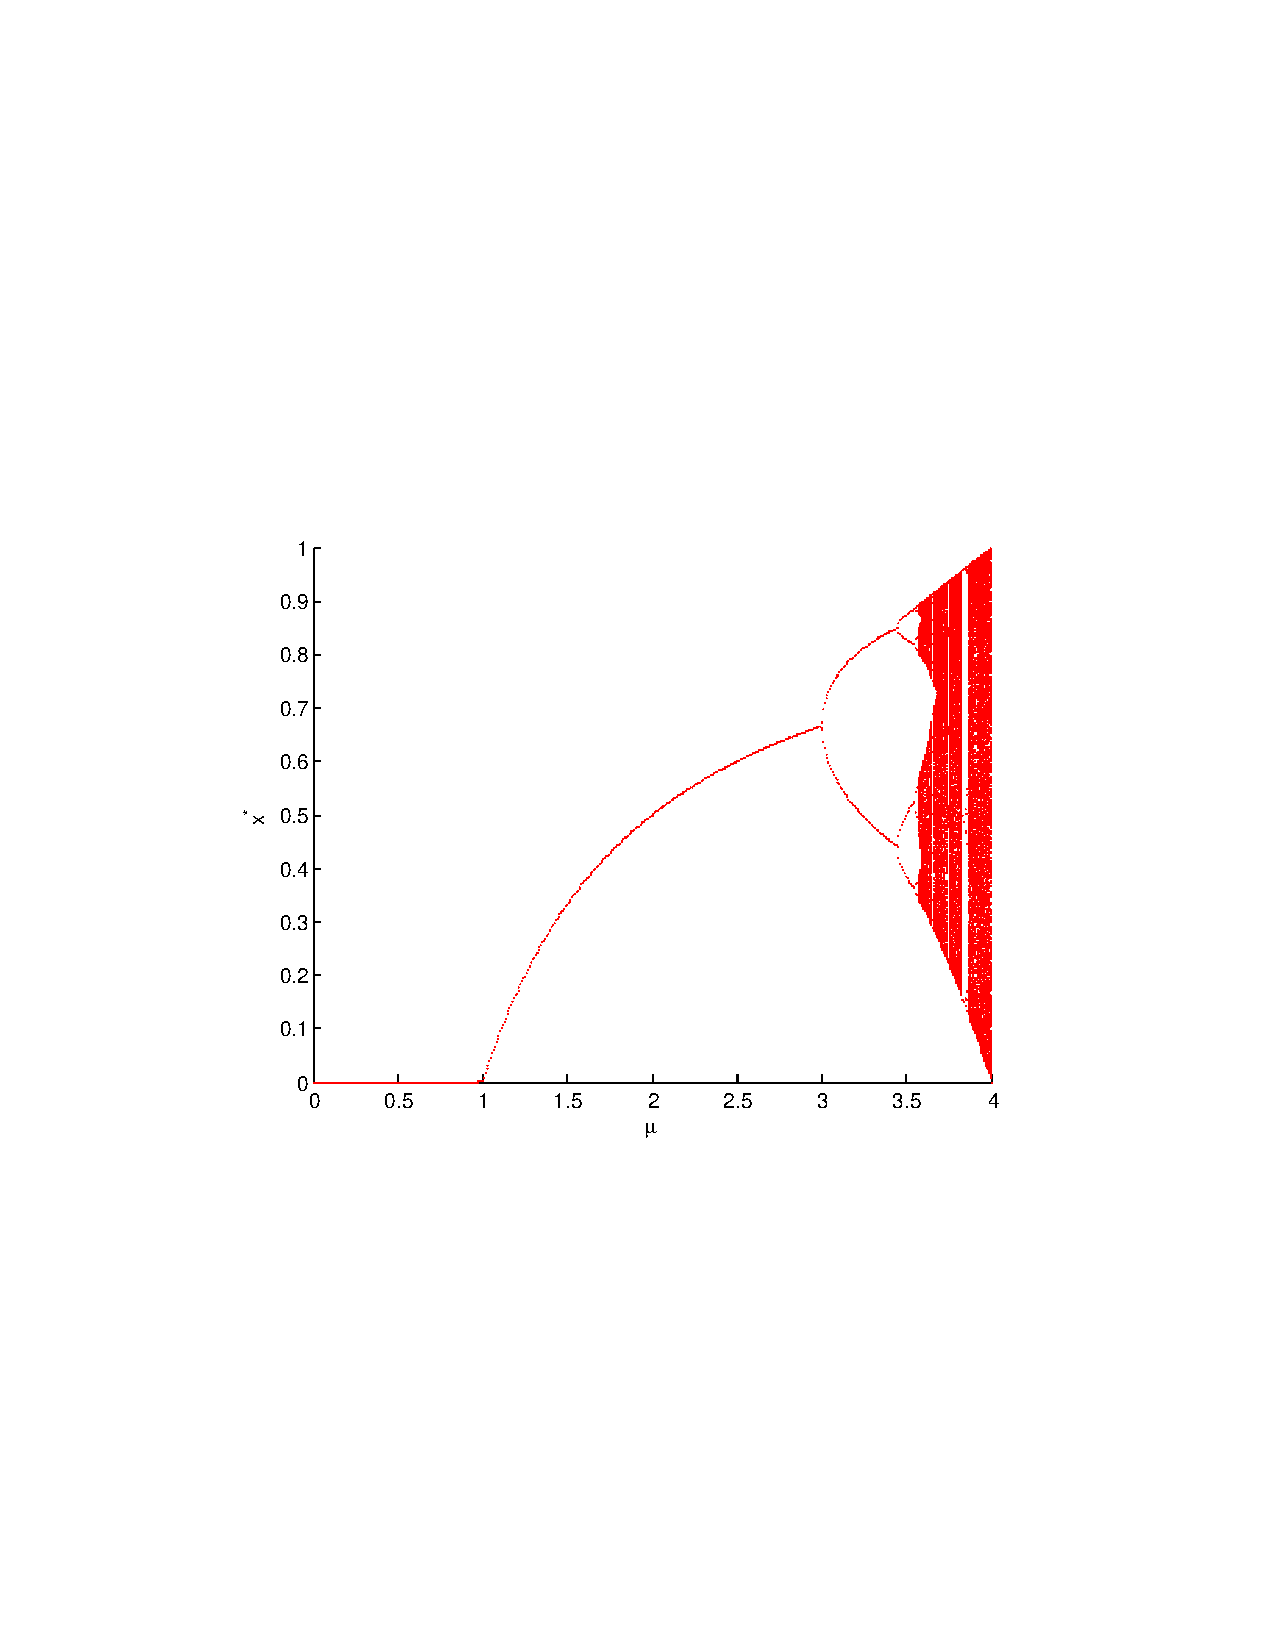
\includegraphics[width=0.9\textwidth]{cascade_full}
\end{center}
}



\section{Conclusion}

\frame{\frametitle{A word of caution}
We have used three different modelling paradigms to describe the growth of a population in a \textbf{logistic} framework:
\begin{itemize}
\item The ODE version has monotone solutions converging to the carrying capacity $K$.
\item The DDE version has oscillatory solutions, either converging to $K$ or, if the delay is too large, periodic about $K$.
\item The discrete time version has all sorts of behaviors, and can be chaotic.
\end{itemize}
It is important to be aware that the {\bf choice of modelling method} is almost {\bf as important} in the outcome of the model as the precise formulation/hypotheses of the {\bf model}.
}

%\section{Critic of the logistic equation in the US census case}
%
%\frame{\frametitle{What is wrong with the logistic equation here?}
%\begin{itemize}
%\item The carrying capacity is constant.
%\item The model does not take immigration into account (for the US, this is an important component).
%\end{itemize}
%}
%
%
%\section{Population curves -- Gompertz}
%
%\frame{
%\begin{center}
%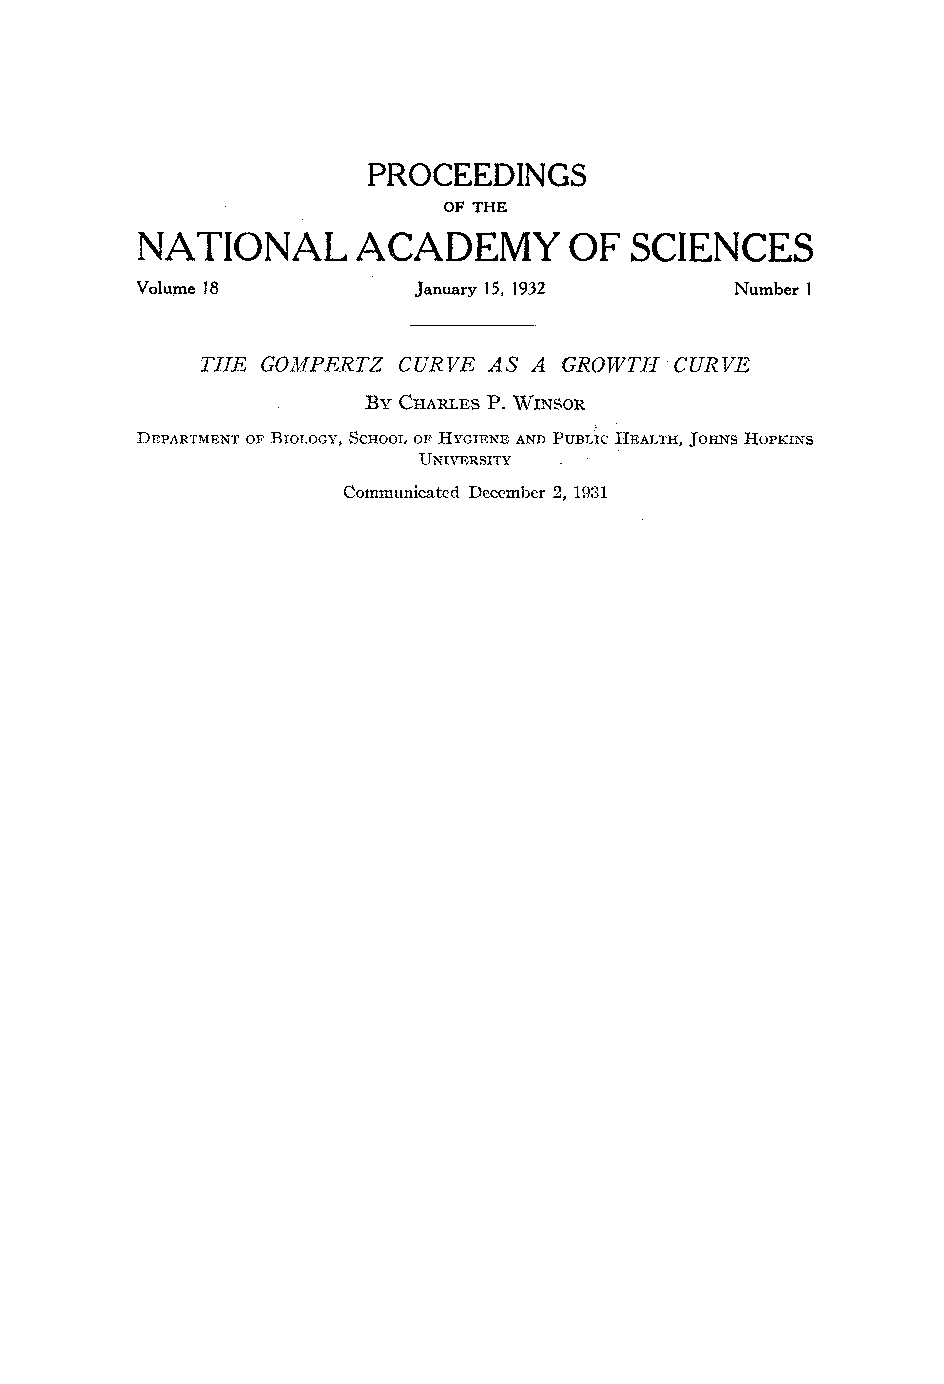
\includegraphics[width=0.95\textwidth]{title_Winsor1932PNAS18}
%\end{center}
%}
%
%\frame{
%\begin{center}
%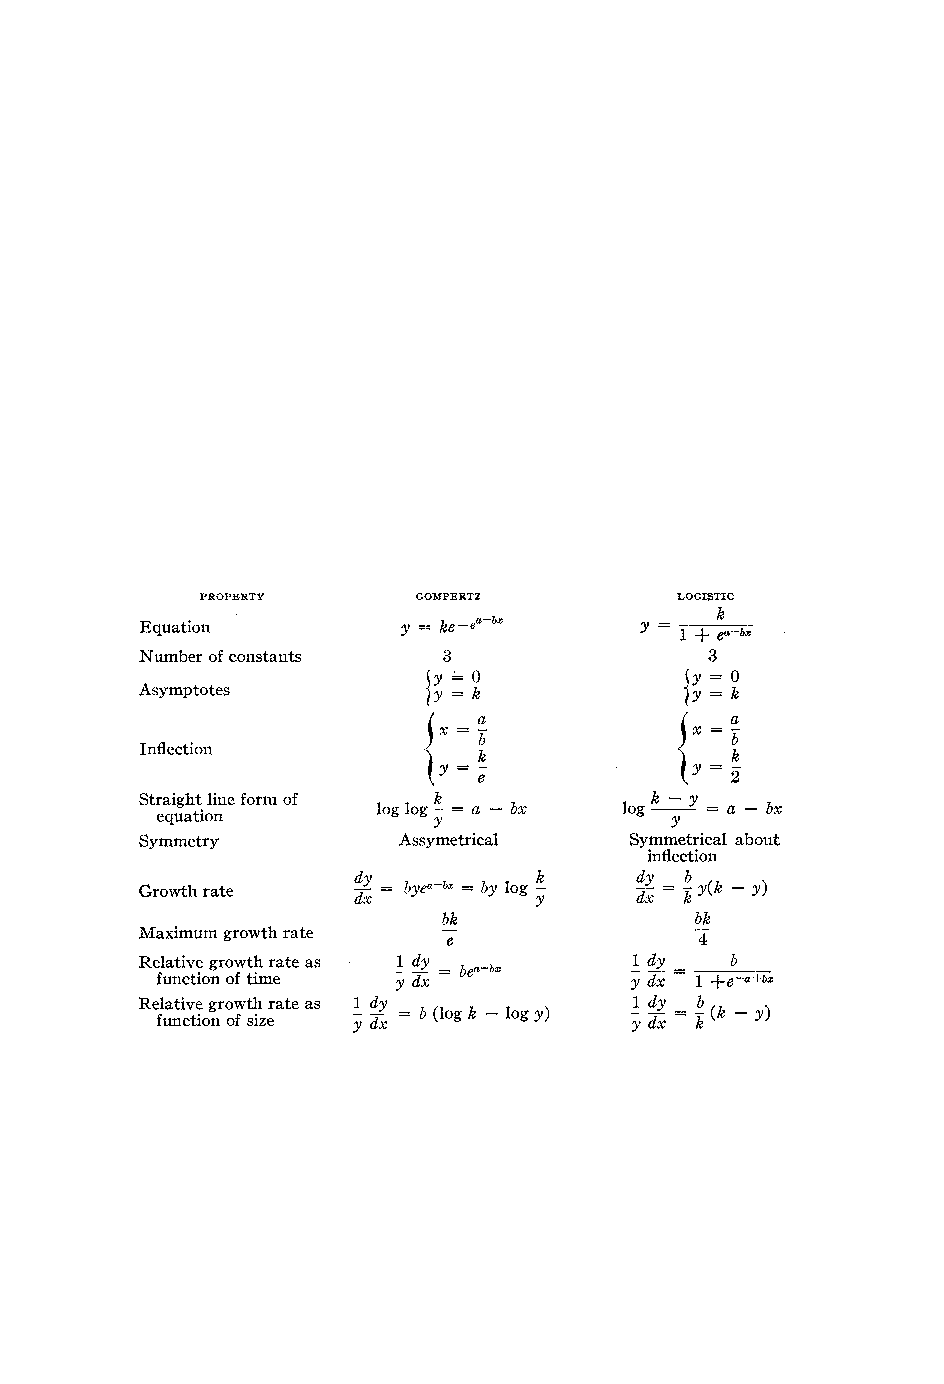
\includegraphics[width=0.95\textwidth]{table_Winsor1932PNAS18}
%\end{center}
%}
%


\end{document}
